\documentclass[colophon, english]{phduio}

\usepackage{phdstyle}   % Custom style
\usepackage{kantlipsum} % Dummy text
\usepackage{tikz-cd} 
\DeclareMathOperator{\tr}{tr}
\DeclareMathOperator{\Tr}{Tr}
\DeclareMathOperator{\Var}{Var}
\DeclareMathOperator{\argmin}{argmin}
\DeclareMathOperator{\Cor}{Cor}
\DeclareMathOperator{\Cov}{Cov}
\DeclareMathOperator{\diag}{diag} 
\DeclareMathOperator{\argmax}{argmax}
\DeclareMathOperator{\supp}{supp}
\DeclareMathOperator{\pa}{pa}
\DeclareMathOperator{\sd}{sd}
\DeclareMathOperator{\dom}{dom}
\DeclareMathOperator{\Lomax}{Lomax}
\DeclareMathOperator{\GammaDist}{Gamma}
\DeclareMathOperator{\Exp}{Exp}

\makeatletter
\numberwithin{equation}{section}
\numberwithin{figure}{section}
\theoremstyle{plain}
\newenvironment{lyxlist}[1]
	{\begin{list}{}
		{\settowidth{\labelwidth}{#1}
		 \setlength{\leftmargin}{\labelwidth}
		 \addtolength{\leftmargin}{\labelsep}
		 \renewcommand{\makelabel}[1]{##1\hfil}}}
	{\end{list}}
\makeatother


\author{Jonas Moss}
\title{Statistics in psychology}
\department{Department of Mathematics}
\faculty{Faculty of Natural Science}
\ISSN{1234-5678}           % Request correct number from repro@uio.no
\dissertationseries{Femme Fatale}  % Request correct number from repro@uio.no


% \includeonly
% {
%     sections/dedication,
%     sections/preface,
%     sections/papers,
%     sections/introduction,
%     sections/chapter2,
%     sections/chapter3,
%     sections/chapter4,
%     sections/appendixA,
%     sections/appendixB,
% }


\begin{document}

    \frontmatter        % Folios in Roman numerals, unnumbered chapters.

    \uiotitle

    %\thispagestyle{empty}
\vspace*{\stretch{1}}
\begin{flushright}
    \emph{To Asbjørg Gjertsen and Gjert Kristian Gjertsen}
\end{flushright}
\vspace*{\stretch{3}}
    \section*{Acknowledgements}

Riccardo De Bin

Thanks to my co-supervisor Nils Lid Hjort. While we did not work much together on this thesis, your influence from the master thesis is strongly felt.

I am grateful to my coauthors. Especially Steffen Grønneberg, the unofficial third advisor of this thesis. It was a pleasure writing the partial identification paper with you and Njål Foldnes! And thanks to Martin Tveten, an excellent partner in \texttt{R}-package development. 

Sven Ove Samuelsen for being a pleasant boss and frequently correcting my misconceptions. Stephan Michelis, for his encouragement and great comments about the \textit{p}-hacking paper. 

Jonas Christoffer Lindstrøm. We have spent countless hours discussing statistics, often directly influencing this, usually over a couple of beers, and often together with Céline Cunén. Emil Stoltenberg, for many deep discussions, particularly about Bayesian statistics, and reading through the infinite confidence interval paper. Vinnie Ko for being an inspiration in getting things done and double-checking some maths in the standardized alpha paper.

Kjersti Moss, for fixing much of my bad writing and listening to me going on and on about esoteric and fundamentally uninteresting topics.

Olav Dovland, my mentor in mathematics the last 10 years or so.

Moreover, I would like to express my appreciation of the members the causality reading group. We didn't get around to write a paper, but I hope we will in the future. The members of the Psychological Methods Research Group should not be left out. Posts in this group were the seeds of two papers in this thesis and two papers that are not finished yet. 

\vskip\onelineskip
\begin{flushleft}
    \sffamily
    \uiocolon\textbf{\theauthor}
    \\
    Oslo,\MONTH\the\year
\end{flushleft}
    \chapter{List of Papers}


\section*{Academic papers}
\begin{enumerate}

\item Moss, J. ``Please avoid the standardized alpha and the ordinal alpha''
(2020). \emph{Submitted for publication.}

\item Grønneberg, S., Moss, J., Foldnes, N. ``Partial identification of
latent correlations with binary data'' (2020). \emph{Invited to resubmit, major revision, Psychometrika.}

\item Moss, J., De Bin, R. ``Modelling publication bias and \emph{p}-hacking''
(2020), \emph{Invited to resubmit, major revision, Biometrics.}

\item Moss, J. ``Infinite confidence intervals in Hedges' model of publication
bias'' (2020). \emph{Submitted for publication.}

\item Moss, J. ``Back-of-the-envelope methods for correcting for \emph{p}-hacking
and publication bias'' (2020). \emph{Manuscript.}
\end{enumerate}

\section*{Software papers}
\begin{enumerate}
\item Moss, J. (2019). univariateML: An R package for maximum likelihood
estimation of univariate densities. J\emph{ournal of Open Source Software},
\emph{4}(44), 1863.
\item Moss, J., \& Tveten, M. (2019). kdensity: An R package for kernel
density estimation with parametric starts and asymmetric kernels.
\emph{Journal of Open Source Software}, \emph{4}(42), 1566.
\end{enumerate}


    \cleartorecto
    \tableofcontents    % Or \tableofcontents*
    \cleartorecto
    \listoffigures      % Or \listoffigures*
    \cleartorecto
    \listoftables       % Or \listoftables*

    \mainmatter         % Folios in Arabic numerals, numbered chapters.
    \chapter{Setting the scene}
    \section{Introduction}

You are reading a statistics thesis about statistics in psychology. Statistics in psychology comes in two packages, and this thesis touches both them.

\textbf{Psychometrics.} What is intelligence, and how do we measure it? How many personality traits are there, and how do they matter? Psychometrics is the science of psychological measurement. There are two kinds of psychometricians; the theoretical and practical. Theoretical psychometricians are just like statisticians, they deal with mathematics and programming. They publish in journals such as \textit{Psychometrika}, \textit{British Journals of Mathematical Psychology}, and \textit{Multivariate Behavioural Research}. These journals are specialized methodological journals, and allow the use of mathematics. Practical psychometrians design measurement instruments and administer them. They publish both in specialized psychometrics journals such \textit{Psychological Assessment}, and methodologically generalist psychology journals such as \textit{Emotion.} The section on psychometrics shows the main models of psychometrics, discusses some fundamental questions, and gives an intuition for what questions we are dealing with and why they matter.

\textbf{Psychological~methods.} Psychological methodology is much wider in scope, encompassing everything that has anything to do with psychological research. Should you use frequentist hypothesis tests, Bayes factors, or maybe avoid testing altogether? When is Pearson's correlation coefficient more appropriate than Spearman's rho? When would multilevel modeling be appropriate? How can you do a high-quality meta-analysis? Pretty much of all applied statistics is relevant to psychologists in some way, and research in statistics is published in psychology journals such as the generalist journals \textit{Psychological Bulletin} and \textit{Psychonomic Bulletin Review}, and the psychological methodology journals \textit{Advances in Methods and Practices in Psychological Science}, and \textit{Psychological Methods}. Psychology is undergoing a replication crisis, and has done so since about $2011$. That was the year when \cite{Bem2011-vq} published his study on paranormal stuff in the top-tier \textit{Journal of Social and Personality Psychology} and \cite{simmons_false-positive_2011} published their famous \textit{False-Positive Psychology} paper. The issue can be summed up like this: You can't trust what psychologists say. Partly due to the replication crisis, psychology is undergoing a reproducibility revolution. The section open science is about what this entails for psychology specifically, and the role of $\mathtt{R}$
and how open science should affect the field of statistics. 

Aside from the psychological context and open science, this thesis discusses two issues not every statistician is familiar with, impossibility results in frequentist estimation and partial identifiability. The section on statistical inference discusses some of the pros and cons of Bayesian and frequentist statistics, and remind the reader about some definitions they might not use that much. Problems involving partial identifiability are everywhere. Whenever you hear someone say something like ``we let $\theta=1$ to make the problem identified,'' chances are you you are facing a tucked-away partial identification problem. And the final section of is about partial identifiable, illustrated with several examples. 
    \section{Statistical inference}

Bayesians are in a privileged position vis-à-vis frequentists. Any problem
has a unique solution for a Bayesian provided he can answer three
questions \parencite[Chapter 2]{Robert2007-ri}:
\begin{enumerate}
\item "What is the structure of reality?" He needs a likelihood for the problem. 
\item "What do I know about reality?" He needs a prior for the parameters
of the likelihood.
\item "What do I want to do, or what to I want to know?" He needs a loss function
to quantify the consequences of choosing the wrong act.
\end{enumerate}
The Bayesian does not only claim that every problem has a unique solution.
His claim is much stronger. Given a likelihood, a prior, and a loss
function, it is \emph{irrational} to do anything else than minimizing
the expected loss, also known as the risk, defined as
\begin{equation}
\argmin_{a\in\mathcal{A}}E[l(X,a)\mid\textrm{data}].\label{eq:risk minimization}
\end{equation}
Frequentist seldom have this luxury. Sometimes solutions with desireable
features do not exists, sometimes it is hard to find candidate confidence
set, sometimes optimality criteria do not hold. Since frequentist
methods usually aren't unique, frequently based on intuition, and
can be based on severely conflicting criteria, they are famously called \emph{ad hoc
methods}. \textcite[p. xxiii]{Jaynes2003-ky} speaks for many Bayesians
in his diatribe against frequentist statistics:
\begin{quote}
{[}F{]}requentist methods provide no technical means to eliminate
nuisance parameters or to take prior information into account, no
way even to use all the information in the data when sufficient or
ancillary statistics do not exist. Lacking the necessary theoretical
principles, they force one to \textquoteleft choose a statistic\textquoteright{}
from intuition rather than from probability theory, and then to invent
ad hoc devices (such as unbiased estimators, confidence intervals,
tail-area significance tests) not contained in the rules of probability
theory.
\end{quote}
The case for Bayesianism is extremely strong \parencite{Berger1988-ji,Bernardo2009-wv}.
But the arguments hinge on the assumption that we know the likelihood,
prior, and loss. Is this realistic? We will consider them in turn. 

The nature of Bayesian inference sometimes requires us to specify
much more than a frequentist needs to. A Bayesian always needs to
specify a prior, and the difficulties involved in finding good priors
takes up a large chunk of the arguments of frequentists against Bayesians,
and has inspired much work in objective Bayes. Getting the benefits
of Bayesian analysis without a using priors has even been called ``holy
grail of statistical theory'' by \textcite{Efron2010-is}. 

But the Bayesian also has to specify a likelihood. In most frequentist
statistics we assume a known likelihood, but not always. In particular,
semi-parametric statistics often assumes no likelihood. For instance,
the \textcite{Cox1972-xd} model assumes only a partially known likelihood,
while the maximum score model of \textcite{Manski1975-gl} makes no likelihood
assumptions at all. Moreover, non-parametric methods, such as kernel
density estimation \parencite{Silverman1986-nt} do not involve likelihoods
at all. Curiously, the archetypal non-parametric estimator, the histogram,
can be framed as a maximum likelihood problem, complete with its own
AIC \parencite{Birge2006-nl}. But even in this case, no likelihoods are
actually assumed. The histogram is just a handy device to estimate
an unknown density. That said, most semi-parametric and non-parametric
problems can be formulated into similar non-parametric Bayes models.
For instance, the natural analogue of kernel density estimation is
the normal Dirichlet mixture model \parencite[Chapter 2.2]{Muller2015-xn}.

But there are problems where Bayesian estimation appears impossible
in principle, namely when the likelihood does not exist.
\begin{example}[{No likelihood, \textcite[p. 30]{Berger1988-ji}}]
\label{exa:no likelihood}Let $\{P_{\theta}\},\,\theta\in[0,1]$
be a parameterized class of probability distributions on $[0,1]$
defined by
\begin{equation}
P_{\theta}(A)=\frac{1}{2}[\lambda(A)+1_{A}(\theta)],\label{eq:no likelihood}
\end{equation}
for all $A$ in the Borel $\sigma$-algebra of $[0,1]$. Here $\lambda$
is the Lebesgue measure. Then $\{P_{\theta}\}$ is not dominated by
any $\sigma$-finite measure. To see why, assume $Q$ dominates $\{P_{\theta}\}$,
that is, $Q(A)\geq P_{\theta}(A)$ for all $\theta$ and all $A$.
In particular, $Q(\theta)\geq1$ for all $\theta\in[0,1]$. By $\sigma$-additivity,
$Q(A)$ is finite if and only if $A$ is finite, and since a countable
union if finite sets is countable, $Q$ is not $\sigma$-finite.
\end{example}

Since $\{P_{\theta}\},\,\theta\in[0,1]$ has no likelihood, the Bayesian
is lost. He might have a prior on $\theta$, for instance a $\textrm{Beta}(2,2)$,
but that does not help him. He might want to use the quadratic loss
function, but he can't. Perhaps he could ditch the idea of likelihoods
altogether and use a predetermined countable partitioning of $\Omega$
instead. But such a solution is most definitely \emph{ad hoc}, and
hard to reconcile with his prior on $\theta$. The only coherent way
seems to be the adoption of a prior with countable support, so that
$\{P_{\theta}\}$ becomes dominated; but then the estimator will be
inconsistent for all $\theta$ outside of that countable support.

On the other hand, the frequentist has no trouble dealing with this
example. There are reasonable estimators for $\theta$ when we observe
repeatedly from $P_{\theta}$. Most obviously, the estimator $\hat{\theta}=a$
if and only if $a$ has been observed at least twice. Confidence sets,
convergence rates, and other frequentist properties are trivially
calculated from this estimator.

An even stranger is case $P_{\theta}(A)=1_{\theta}(A)$. Here $\theta$
is uniquely identified from a single observation, but has no likelihood,
and no Bayesian analysis is possible.

These two examples don't look realistic at all, and might be brushed
aside as mere curiosities. A more practically serious problem appears
when a likelihood appears to exist, is hard to reason about, but is
somehow not needed for the problem.
\begin{example}[Robins--Ritov--Wasserman]
 This example due to \textcite{Robins2012-fr}. We will consider a sequence
of $n$ independent and identically distributed variables $(X_{i},Y_{i},Y_{i}^{*},R_{i})$,
where $X_{i}\in[0,1]$ is uniform,  $R_{i}$ is binary, $Y_{i}^{*}\in\{0,1\}$,
and $Y\in\{\textrm{NA},0,1\}$. Here $Y_i^{*}$ are unobserved; instead
of observing $Y_{i}^{*}$, we observe
\[
Y=\begin{cases}
Y^{*}, & R=1,\\
\textrm{NA}, & R=0.
\end{cases}
\]
Here $R$ is allowed to depend on $X$, with \emph{known} conditional
probability $\pi(x)=p(r=1\mid x)$. The joint density of $(X,Y,R$) is
\begin{eqnarray*}
p(x,y,r\mid\theta) & = & \begin{cases}
p(y\mid x,\theta)\pi(x), & r=1,\\{}
[1-\pi(x)]1\{y=\textrm{NA}\} & r=0.
\end{cases}
\end{eqnarray*}
Our goal is to estimate $\psi=P(Y_{i}^{*}=1)=\int p(y\mid x,\theta)dx$.
We do not wish to assume any specific parametric form for the true
$p(y\mid x,\theta)$. Anyhow, the posterior is proportional to
\begin{eqnarray*}
p(\theta\mid\textrm{data}) & \propto & \prod_{r_{i}=1}p(y\mid x_{i},\theta)\pi(x_{i})\prod_{r_{i}=0}1\{y=\textrm{NA}\}(1-\pi(x)),\\
 & \propto & \prod_{r_{i}=1}\pi(x_{i})\prod_{r_{i}=1,}p(y\mid x_{i},\theta).\\
 & \propto & \prod_{r_{i}=1,}p(y_{i}\mid x_{i},\theta).
\end{eqnarray*}
Hence the posterior does not depend on $\pi(x)$ unless the prior
does. However, \textcite{Robins1997-uv} proved that any uniformly consistent
estimator of $\psi$ must depend on $\pi(x)$. In this sense, any Bayesian estimator of $\hat{\theta}$ is inadequate. No matter what likelihood and prior you choose, the estimator of $\psi$ won't be uniformly consistent.

On the other hand, there is a well-known uniformly consistent estimator of $\psi$,
namely the \emph{Horwitz--Thompson} estimator
\begin{equation}
\hat{\psi}=\frac{1}{n}\sum_{i=1}^{n}\frac{Y_{i}R_{i}}{\pi(X_{i})}.\label{eq:Horwitz-Thompson}
\end{equation}
It is unbiased, and it variance shrinks to $0$ as $n\to\infty$,
hence it's consisent. Moreover, the interval $C=\{\hat{\psi}\pm([2n\delta^{2}]^{-1}\log(2/\alpha))^{1/2}\}$
is a valid finite sample level $\alpha$ confidence set, i.e.
\[
P(\psi\in C)\geq1-\alpha\quad(P\in\mathcal{P})
\]
for all $n$.
\end{example}

The Robins--Wasserman does not matter to a Bayesian that firmly knows the likelihood and the prior. For him, the Bayes' theorem is the best you could possible do. And by Doob's consistency theorem \parencite{Miller2018-xq}, if you know your prior is true, every Bayesian procedure is consistent.

The Bayesians that are troubled by this example are the bounded Bayesians, those who have only limited trust in their
priors and likelihoods, and try to make do with approximations. In
parametric problems, the bounded Bayesians are relatively safe. Due
to the Bernstein--von Mises phenomenon \parencite[Section 10.2]{Van_der_Vaart2000-qc},
the prior does not matter in the limit, as $n\to\infty$. Moreover,
parameter estimates such the posterior mean will converge to the do
the Kullback--Leibler-minimizing parameter \parencite[Theorem 2.1]{Bunke1998-vg},
sometimes called least-false parameters \parencite[p. 25]{Claeskens2008-hk},
just as they do for maximum likelihood estimation.

But non-parametric Bayesians doesn't have the luxury of an unconstrained
Bernstein--von Mises phenomenon. The imaginary logical omniscience
of the Bayesian has practical consequences now. In the Robins--Wasserman
example, the frequentist is luckier than the Bayesian, as he does
not have pretend to be omniscient at all. He does not need to pretend
to know the likelihood $p(y\mid x,\theta)$, much less a prior for
it. The Horwitz--Thompson estimator is an empirical average, not
a function of the likelihood.

As a Bayesian who admits not to be logically omniscient, what should
you do? The frequentist method suggests a possible solution. We are
looking for an esimator of the mean $\psi$, but the theoretical Bayesian
is forced to supply a likelihood for the far more general $\theta$.
But we can reformulate the problem so $\theta$ does not appear at
all. 
\begin{example}[Response to Robins--Wasserman]
 The bounded Bayesian will not know the likelihood of $\theta$,
but there is still hope for him, as he has some information about
the problem. In particular, he knows that $E[Y_{i}R_{i}/\pi(X_{i})]=\psi$.
As any statistician worth his salt, he pretends that $Y_{i}R_{i}/\pi(X_{i})$
is normal. He can then use e.g. a normal prior for the mean parameter
of this normal distribution, and analyze it as an ordinary normal-likelihood
and normal-prayer Bayesian problem.
\end{example}

\textcite{Sims2012-ze} proposes other bounded Bayesian solutions
to the Robins--Ritov--Wasserman problem. Wasserman and Robins interprets
such solutions as engaging in \emph{frequentist persuit}. That is,
an attempt to manipulate Bayesian procedures to have good frequentist
properties through \emph{ad hoc} metods. But the bounded Bayesian
does not do his analysis due to frequentist persuit. He does it because
he is aware of his own ignorance: No one can force you to know something
you don't, and you don't know the likelihood of $y\mid x$, much less
its prior. The bounded Bayesian retains some of his upper hand vis-à-vis
the frequentist, as he is able to incorporate his knowledge about
$\psi$ into his prior and has guaranteed frequentist properties via
the Bernstein--von Mises theorem.

That said, plenty of self-declared Bayesians are happy to engange
in frequentist persuit. In this section, ``Bayesian'' is used in
the sense of Finetti and Savage, as an ideal, rational actor. Most
Bayesians are not dogmatic in this sense, but pragmatic Bayesians
who use the methods because they often work better than frequentist
methods. For instance, \textcite{Gelman2013-ib} argue that the Bernstein--von Mises
phenomenon is essential to the Bayesian because it guarantees good frequentist properites of confidence sets. (On the other hand, \textcite{Morey2016-ry} argue that confidence sets are worthless unless they can be given a Bayesian interpretation.)

\subsection{Loss functions}

Loss functions don't receive much attention at all. Most statisticians
let $l$ be quadratic, the action space be the parameter space, and
call it a day. While this procedure certainly is practical, it's hard
to defend philosophically. Loss functions can be categorized into
at least five classes, depending on their actions space.
\begin{lyxlist}{00.00.0000}
\item [{\textbf{Point~prediction}}] Our goal is to predict the value of
a new sample of $X$. In this case, the action space $\mathcal{A}$
has to be a subset of $\dom X$, the domain of $X$. The loss function
is $l(a,x)=E_{X\mid\theta}[l'(a,x)]$, where $l'(a,x)$ should equal
$0$ if and only if $a=x$, and $l'(a,x)>0$ for all other $a\in\dom X$.
Well-known prediction losses of this kind are the $L_{p}$-losses,
$l'(a,x)=|a-x|^{p}$, the $0-1$-loss $l'(a,x)=1[a=x]$, the Linex
loss $l'(a,x)=b(e^{c(x-a)}-c(x-a)-1)$ \parencite{Varian1975-cd}, and
the Huber loss from robust statistics \parencite{Huber1964-fm}. For all
of these cases, the risk $R=\min_{a\in\mathcal{A}}E[l(a,x)]$ tells
you how certain you can be about your prediction of $X$.
\item [{\textbf{Density~prediction}}] The action space $\mathcal{A}$
is a subspace of the space of densities on $\mathcal{X}$. Again,
we should demand that $l(g,f)=0$ if and only if $g=f$ a.e., and
$l(g,f)>0$ for all other $g$. That is, $l$ is a statistical divergence
function. Some well-known divergences are the Kullback--Leibler divergence,
the $L_{2}$-divergence, the Hellinger distance, and the class of
$f$-divergences \parencite{Basu2011-gs}. 
\item [{\textbf{Parameter~estimation}}] The action space $\mathcal{A}$
is a subset of the parameter space $\Theta$. The loss function will
have the same properties as in point prediction, i.e., the loss $l(a,\theta)$
should equal $0$ if and only if $a=x$, and $l(a,x)>0$. The by far
most popular loss is the quadratic loss. The context is usually stated
as ``parameter estimation'', without any more details about the
problem or a statement as to why you should be interested in the parameters
themselves.
\item [{\textbf{Instrumental~losses}}] Sometimes we design our loss functions
to help us reach our statistical goals. One application is the formulation
of stopping rules in sequential analysis \parencite{Brockwell2003-pd}.
A natural stopping rule is to check the posterior risk, continue if
it is too large, and stop if it is too small. We add an increasing
penalty $C_{k}$ to the loss, where $k$ is the sample size, since
sampling costs money. The action space is the product two spaces.
The first space contains two actions, Stop and Continue. If the action
chosen is Stop, we will stop our sampling process; if it is Continue,
we will continue the sampling process. The second space is $\dom X$,
and the risk is $E_{X\mid\textrm{data}}[l(\mu,X)]+C_{k}$. Similar
instrumental losses can be used for e.g. sparse estimation.
\item [{\textbf{Practical~losses}}] Much decision theory is framed in
terms of practical losses but they are rarely used. A practical loss
is simply a loss that doesn't fit into the categories above. For example,
\textcite{Stankovic1985-th} employs custom-made loss for the problem
of decentralized control of job scheduling. 
\end{lyxlist}
The parameter estimation losses are not well-motivated. It's hard
to imagine any situation where anyone would directly care about the
posterior mean of $\mu$, philosophically speaking. Yes, posterior
means and standard deviations are easy to calculate and intertrep,
but this is hardly a deep justification to employ them. Losses on the parameter space does not take into account that parameterizations are, in a sense, arbitrary. For any identified $k$-dimensional parameterization of a likelihood, there are $2^{\mathfrak{c}}$ (where $\mathfrak{c}$ is the cardinality of the continuum) identified $k$-dimensional parameterizations, and why care only about one of them? 

For a better motivated variant of parameter estimation, we could re-frame the problem as a density estimation problem. For if let let the action space $\mathcal{A}$ be the space of likelihoods, we are essentially dealing with a \emph{parameterization-agnostic} estimation problem. 
\begin{example}
\label{exa:exponential estimation} Let $X_{1},\ldots,X_{n}\sim\Exp(\lambda)$
and $\lambda\sim\GammaDist(\alpha_{0},\beta_{0})$. It is well-known
that the posterior distribution is $\GammaDist(\alpha,\beta)$, with
parameters $\alpha=\alpha_{0}+n$, $\beta=\beta_{0}+n\overline{x}$.
The posterior predictive distribution is $\Lomax(\alpha,\beta)$,
which has density $\alpha\beta^{\alpha}(x+\beta)^{-\alpha-1}$. 

A popular way to do density prediction is to use the the posterior
predictive density. This\emph{ }is the point-wise solution to the
risk-minization problem $\min_{p}E_{\theta\mid\textrm{data}}\{[p(x)-f_{\theta}(x)]^{2}\}$,
where $f_{\theta}(x)$ is the aleatoric density at a data point. But
this density is not decision-theoretically justified; it is merely
a marginalized density. To justify the usage of the posterior predictive
density, we need a loss function over over the space of densities, as described above.
The best-known and most popular such loss function is the Kullback--Leibler\emph{
}divergence \parencite{Kullback1951-kv}
\begin{equation}
d_{KL}(f,g)=\int\log\left[\frac{f(x)}{g(x)}\right]f(x)dx.\label{eq:Kullback-Leibler}
\end{equation}
 Define the \emph{entropy} $H(f)=\int-\log[f(x)]f(x)dx$ and the \emph{cross-entropy}
$H(f,g)=-\int\log[g(x)]f(x)dx$. Assuming finite entropy and cross-entropy,
\begin{equation}
d_{KL}(f,g)=H(f,g)-H(f).\label{eq:Kullback--Leibler(entropy)}
\end{equation}
Provided $E_{\theta\mid\textrm{ data}}[H(f_{\theta})]$ is finite,
the posterior predictive distribution $\tilde{p}$ solves $\min_{p}E_{\theta\mid\textrm{data}}[d_{KL}(f_{\theta},p)]$.
That is, $\tilde{p}=\argmin_{p\in\mathcal{P}}E_{\theta\mid\textrm{data}}[d_{KL}(f_{\theta},p)],$
where $\mathcal{P}$ is the space of all densities. To see why, observe
that
\begin{eqnarray}
 &  & E_{\theta\mid\textrm{data}}\left(\int[\log f_{\theta}(x)-\log(g)]f_{\theta}(x)dx\right)\nonumber \\  
 & = & E_{\theta\mid\textrm{data}}[H(f_{\theta},g)]-E_{\theta\mid\textrm{data}}[H(f_{\theta})],\label{eq:cross-entropy equality}\\
 & = & H(\tilde{p},g)-E_{\theta\mid\textrm{data}}[H(f_{\theta})],\nonumber 
\end{eqnarray}
and that this is minimized in $g=\tilde{p}$, as the true distribution
minimizes the cross-entropy. 

Parameter estimation can be framed in similar terms. Estimating the
parameters of a density $f$ is just a rephrasing of estimating the
density. That is, estimating the $\lambda$ parameter in an
exponential model is the same kind of problem as estimating $f_{\lambda}$,
the exponential density itself. Now let $\mathcal{P}$ the family
of exponential densities . Then $\argmin_{p\in\mathcal{P}}E_{\theta\mid\textrm{data}}[d_{KL}(f_{\theta},p)]$,
an estimate of the density $f_{\lambda}$, can readily be calculated.
This method of estimating parameters is studied by \textcite{Robert1996-ii},
who calls the statistical divergences intrinsic losses. 

From the equations (\ref{eq:cross-entropy equality}) above, we know
we only have to minimize the cross-entropy $H(\tilde{p},g)$. Let
$X\sim\Lomax(\alpha,\beta)$, then calculate
\begin{eqnarray*}
H(\tilde{p},g_{\lambda}) & = & \int[\log\lambda-\lambda x]\alpha\beta^{\alpha}(x+\beta)^{-\alpha-1}dx,\\
 & = & \log\lambda-\lambda EX=\log\lambda-\lambda\frac{\beta}{\alpha-1}.
\end{eqnarray*}
This function reaches its minimum in $\hat{\lambda}_{KL}=(\alpha-1)/\beta$,
where $H(\tilde{p},g_{\lambda})=\log\beta-\log(\alpha-1)$. Compare
this to the posterior mean, which for this particular parameterization
is the slightly larger $\alpha/\beta$. 

Recall that maximum likelihood estimation can be formulated in terms
of Kullback--Leibler minimization \parencite[p. 25]{Claeskens2008-hk}:
If $F_{n}$ is the the empirical cumulative distribution function,
the maximim likelihood estimator is $\hat{\theta}_{ML}=\argmin d_{KL}(F_{n},f_{\theta})$.
Since $\hat{\theta}_{ML}$ is invariant under reparameterizations
(just like other minimum distance estimators, see \textcite{Drossos1980-ar}),
it is hardly surprising that the Kullback--Leibler loss minimizer
is invariant under reparameterizations too. 
\end{example}


\subsection{Frequentist statistics}

Frequentist inference is hard to understand for lay people. Misunderstandings
about \emph{p}-values and confidence intervals are ubiquitous, documented
in fields such as psychology \parencite{Belia2005-di,Gigerenzer2018-oi}
and medicine \parencite{Goodman2008-ed,Gigerenzer2007-qi}. Frequentist quantities are almost never unique in the same
sense as Bayesian quantities, and they are often hard to reason about
mathematically. 

The much harder mathematics involved in research level frequentist
statistics has led to an understanding that Bayesian statistics is
boring. 
\begin{quote}
What is the principal distinction between Bayesian and classical statistics?
It is that Bayesian statistics is fundamentally boring. There is so
little to do: just specify the model and the prior, and turn the Bayesian
handle. There is no room for clever tricks or an alphabetic cornucopia
of definitions and optimality criteria. I have heard people who should
know better use this 'dullness' as an argument against Bayesianism.
One might as well complain that Newton's dynamics, being based on
three simple laws of motion and one of gravitation, is a poor substitute
for the richness of Ptolemy's epicyclic system. \parencite{Dawid2000-aw}
\end{quote}
It's easy to forget just how strange hypothesis tests, confidence
sets, and \emph{p}-values are. 

\subsubsection{Hypothesis tests, \emph{p}-values, and confidence intervals}

In the following pages, $(\Omega,\mathcal{\mathcal{F}})$ will be
a measurable space and $\mathcal{P}$ a backgroud family of probability
measures on this space. The family $\mathcal{P}$ contains every probability
measure we consider plausible. 
\begin{definition}
\parencite[][Chapter 3.1]{Lehmann2005-sp} Let $\mathcal{P}_{0}$ be a family
of probability measures on $(\Omega,\mathcal{F})$. A test of the
null-hypothesis $P\in\mathcal{P}_{0}$ of \emph{size} $\alpha$ is
a set $R$ such that $\sup_{P\in\mathcal{P}_{0}}P(R)=\alpha.$ A test
of $P\in\mathcal{P}_{0}$ of \emph{level $\alpha$ }is a set $R$
such that $\sup_{P\in\mathcal{P}_{0}}P(R)\leq\alpha.$
\end{definition}

The set $R$ is the \emph{rejection set} of the hypothesis test. Its
complement is the acceptance set of the hypothesis and is denoted
$A=R^{c}$. The philsophical underpinning of hypothesis test, due
to Neymann, is that you have to have make a binary choice. Either
you act as if $P\in\mathcal{P}_{0}$ is true, or you act as if $\mathcal{P}_{0}$
isn't true. When you do a hypothesis test, you choose $\mathcal{P}_{0}$
if $\omega\in R^{c}$ and $\mathcal{P}_{1}=\mathcal{P\backslash P}_{0}$,
the alternative hypothesis, otherwise. The definition of hypothesis
test guarantees you will choose $\mathcal{P}_{1}$ when
$\mathcal{P}_{0}$ is true with at most probability $\alpha$. Usually,
discussions of hypothesis tests will involve the probability that
$\mathcal{P}_{1}$ is chosen when $\mathcal{P}_{1}$ is true; this is called the
\emph{power} of the test \parencite{Neyman1977-nx}.

Hypothesis tests are quite easy to understand, especially when formulated
with explicit null-hypotheses and alternative hypotheses. The complexity
goes up a notch with \emph{p-}values.
\begin{definition}
\label{def:p-value}(\textcite[][Chapter 3.3]{Lehmann2005-sp}, \textcite{Bayarri2000-dt}) Let
$A\subseteq[0,1]$ and $R(\alpha)$ be an increasing sequence of size
$\alpha$ rejection sets under $\mathcal{P}_{0}$, i.e., $R(\alpha')\subseteq R(\alpha)$
when $\alpha'\leq\alpha$, and $\sup_{P\in\mathcal{P}_{0}}P(R)=\alpha$.
Then random variable
\begin{equation}
U(\omega)=\inf\{\alpha\mid\omega\in R(\alpha)\}\label{eq:size p-value}
\end{equation}
is a \emph{p}-value. 
\end{definition}

Observe that $U\leq\alpha=\left\{ \omega\mid\inf\{\alpha'\mid\omega\in R(\alpha')\}\leq\alpha\right\} =R(\alpha)$.
Importantly, $U$ satisfies $\sup_{P\in\mathcal{P}_{0}}P(U\leq\alpha)=\sup_{P\in\mathcal{P}_{0}}P(R(\alpha))=\alpha$
for all $\alpha\in A$. When $\mathcal{P}_{0}$ is a singleton, $P(U\leq\alpha)=P(R(\alpha))=\alpha$.
In particular, if $A=[0,1]$, $U$ is uniformly distributed under
$P$, a common definition of a \emph{p}-value in and of itself. The definition
of \emph{p}-value is slightly more general than usual, as it allows
for both $A\neq[0,1]$ and composite hypotheses. The \emph{p}-value
suffers from an all-too-common problem in statistics; there is no
different name for the observed \emph{p}-value $u$ and the \emph{p}-value
statistic $U$. \textcite{Schweder1988-nh} proposed to call $U$ the
``signficance statistic'', a name that has unfortunately not caught
on. 

You could claim this definition of a \emph{p}-value is too convoluted.
But common definitions of\emph{ p}-values are incomplete, most of
them being variants of ``the probability of observing something at
least as extreme as the observed data, given the null hypothesis is
true.'' A better definition is ``the probability of observing $T\geq t$,
where $t$ is a observation of the statistic $T$'', as it makes
the dependence on the (often arbitrary) statistic $T$ explicit. But
stating it in terms of of increasing rejection sets is even better,
as it makes it clear just how many \emph{p}-values there are, how
permissive the definition is, and how the definition is fundmentally
about chains in the $\sigma$-algebra $\mathcal{F}$. Moreover, the
connection between hypothesis tests and \emph{p}-values is easiest to state
and appreciate in terms of rejection sets. The notion of most powerful
\emph{p}-value is obvious; a \emph{p}-value is most powerful against
$\mathcal{P}_{1}$ if each rejection set $R(\alpha)$ is a most powerful
size $\alpha$ hypothesis test. The usual formulation hides this though, stating only $H_0:\mu = 0$, not $H_0:\mu=0,\sigma>0$.

To see why \emph{p}-values should be defined for composite hypothesis,
consider the most famous of test of them all, the two-sided $t$-test.
The null-hypothesis $\mathcal{P}_{0}$ is the family of normal probabilities
with mean zero and any standard deviation $\sigma$, which is composite.
Luckily, $\sqrt{n}\overline{x}/s$ is a pivot in this situation, i.e.,
$P_{\sigma}(\sqrt{n}\overline{x}/s\leq x)$ is independent of $\sigma$,
but the null-hypothesis is still composite. 

How should you use \emph{p}-values for inferential purposes? That's
really hard to say. First of all, notice that a \emph{p}-value does
not have the error-rate interpretation as an hypothesis test. A of
p-value of $0.05$ is not observed with probability $0.05$ under
the null-hypothesis, but a \emph{p}-value of $0.05$ or less is observed
with probability $0.05$. 

It is hard to interpret \emph{p}-values. The definition is opaque and hard, if not impossible, to connect to real-life outcomes. And it is hard to justify the use numbers one cannot expect anyone to interpret in any meaningful way, especially because people will try to interpret it, and inevitably fail. \textcite{Cohen1994-au} wrote, in his critique of \emph{p}-values, 
\begin{quotation}
What's wrong with {[}null-hypothesis significance testing{]}? Well,
among many other things, it does not tell us what we want to know,
and we so much want to know what we want to know that, out of desperation,
we nevertheless believe that it does! What we want to know is \textquotedbl Given
these data, what is the probability that $H_{0}$ is true?\textquotedbl{}
\end{quotation}
Some authors, most famously Fisher \parencite{Liu2020-er} attempt to justify \emph{p}-values
as measures of evidence, and, according to \textcite{Berger1987-tf}
most statisticians use \emph{p}-values since they are ``feeling it
to be important to indicate how strong the evidence against $H_{0}$''.
\textcite{Hubbard2008-cg}, among others, are strongly critical of the
idea that \emph{p}-values are a measure of evidence, but \textcite{Liu2020-er} defend a slight modification of Definition \ref{def:p-value}, incorporating asymptotic guarantees, as being a reasonable measure of evidence.

One reason why \emph{p}-values are not measures is evidence is the lack of explicit alternative hypotheses. That \emph{p}-values are usually framed without explicit alternative hypotheses is sometimes framed as a strength. \textcite[p. 308]{Barnard1962-rz} wrote that ``the simple tests of significance arise ,it seems to me, in situations where we do not have a parameter space of hypotheses; we have only a single hypothesis essentially, and the sample space then is the only space of variables present in the problem.`` Fisher was firmly against formal alternatives hypotheses and power calculations \parencite{Lehmann1993-oa}. A compelling argument for why alternative hypotheses are important is the Albino argument of \textcite{Berkson1942-hj}:
\begin{quotation}
Suppose I said, \textquotedblleft Albinos are very rare in human populations, only one in fifty thousand. Therefore, if you have taken a random sample of 100 from a population and found in it an albino, the population is not human.\textquotedblright{} This is a similar argument but if it were given, I believe the rational retort would be, \textquotedblleft If the population is not human, what is it?\textquotedblright{} 
\end{quotation}
A major difference between the Neyman--Pearson theory of statistical
tests and \textit{p}-values is the theoretical justification. Classical Neyman--Pearson-type
inferential statistics, with Lehmann's ``Testing statistical
hypotheses'' \parencite{Lehmann2005-sp} as its bible, is concerned with
finding optimal tests. Usually, uniformly most powerful tests or uniformly
most powerful unbiased tests do not exist, but it is sometimes possible
to find other kinds of optimal tests. Optimality theory gives you
justification for selecting one test instead of another, and maybe
more importantly, forces you to think clearly about exactly what your
assumptions are and exactly what you want to test. \emph{p}-values,
almost never framed in this way, are much more arbitrary. 

Confidence sets are even harder handle than \emph{p}-values. For while
\emph{p}-values are defined in terms of a nested family of rejection
sets, a confidence set needs a parameterized family of rejection sets.
\begin{definition}
\label{def:confidence sets}Let $\Pi=\{\mathcal{P}(\theta)\}_{\theta\in\Theta}$
be a partition of probabilities on a common probability space $(\Omega,\mathcal{F})$.
A confidence set of level $\alpha$ is mapping $R:\Theta\to\mathcal{F}$,
a family of rejection sets, satisfying 
\begin{equation}
\sup_{\theta\in\Theta}\sup_{P\in\mathcal{P}(\theta)}P(R_{\theta})\leq\alpha\label{eq:confidence set}
\end{equation}
If the inequality is an equality, the confidence set has size $\alpha$. 
\end{definition}

Usually we define a set $C(\omega)$ by $\theta\in C(\omega)\iff\omega\notin R_{\theta}$ and call $C$ a confidence set. The definition above uses the well-known duality between rejection sets and confidence sets, and constructing a confidence set from rejection sets in this way is called
\emph{inverting a test}. The definition might look more abstract than necessary, as it involves two suprema. But both are necessary, despite they not showing up in the most familiar examples. The supremum over $\mathcal{P}(\theta)$ guarantees that that $P(R_{\theta})\leq\alpha$
for every $P$ in the equivalence class $\mathcal{P}(\theta)$, while
the supremum over $\Theta$ guarantees that this is the case for each equivalence class.

A confidence set should be regarded as family of rejection sets, not
as a random set. For it to be random set we would have to find a $\sigma$-algebra
$\mathcal{G}$ over a suitable space of sets $\mathcal{X}$ such that
$C:\Omega\to\mathcal{X}$ is measurable, i.e., $C^{-1}(G)\in\mathcal{F}$
for every $G\in\mathcal{G}$. Luckily, this is unneccessary, as we
are never interested in questions such a ``What is the probability
under $P$ that $C$ is an element of $\mathcal{D}$?''. But a formalization
of $C$ as a random set would would be necessary to answer such questions.

Confidence sets are not only hard to define, they are hard to understand.
You can't figure a handy reformulation of confidence sets, as that
does not exist \parencite{Morey2016-ry}. 
\begin{example}[{\textcite[Example 4a]{Berger1988-ji}}]
 Let $X\in\{1,2,3\}$ and $\theta\in\{1,2\}$. Define

\[
P_{0}(x)=\begin{cases}
0.009, & x=1.\\
0.001, & x=2,\\
0.99, & x=3,
\end{cases},\;P_{1}=\begin{cases}
0.001, & x=1.\\
0.989, & x=2,\\
0.01, & x=3,
\end{cases}
\]
The rejection set $R=\{x\neq3\}$ is the most powerful test of $P_{0}$
vs $P_{1}$, with both error probabilities equal to $0.01$. Now suppose
you observe $x=1$, whereupon you would reject $P_{0}$ in favour
$P_{1}$ according to $R$. But $x=1$ is $9$ times more likely under
$P_{0}$ than under $P_{1}$!
\end{example}

Moreover, confidence sets can be empty; even optimal confidence sets
can be empty \parencite{Blaker2000-ud}. Confidence set for a real parameter
can contain the entire real line \parencite{Morey2016-ry}. Most confidence
sets are asymptotic, but with no guaranteed coverage since uniform
convergence almost never is proved, or even true \parencite{Gleser1996-kk}.

\subsubsection{Impossibility results}

Let's say you have a sequence of real random variables $X_{1},X_{2},\ldots,X_{n}$
from some probability measure $P$ with finite mean $\mu=EX_{1}<\infty$.
You do not know anything else about $P$. Is it possible to say anything
about the mean $\mu$? From a Bayesian perspective the answer is no,
as the problem is underspecified. The problem lacks not only a prior,
but a likelihood too. Even worse, there is no $\sigma$-finite dominating
measure for the class of candidate $F$s, so Bayes' theorem would
be useless in any case. 

But what happens with \emph{p}-values? It turns out there is no nice
\emph{p}-value for the mean, or even hypothesis test, for non-parametric
families of distributions, even when the variance is finite for every
$P$. \textcite{Bahadur1956-tg} proved the following elegant theorem.
\begin{theorem}[Bahadur--Savage]
Let $\mathcal{\mathcal{P}}$ be a family of probability measures
satisfying
\begin{enumerate}
\item[i.)] The expectation $\mu_{F}=\int xdP$ exists and is finite for every
$P\in\mathcal{P}$.
\item[ii.)] For every $\mu\in\mathbb{R}$, there is an $P\in\mathcal{\mathcal{P}}$
satisfying $\mu(P)=\mu$.
\item[iii.)] The family $\mathcal{\mathcal{P}}$ is closed under convex combinations.
That is, if $\lambda\in[0,1]$ and $P,Q\in\mathcal{P}$, then $\lambda P+(1-\lambda)Q\in\mathcal{P}$
too.
\end{enumerate}
Let $\mathcal{P}_{n}(\mu)$ denote the family of probability measures
containing every $P^{n}$ such that $P\in\mathcal{P}$ and $\mu(P)=\mu$.
Let $R$ be a size $\alpha>0$ rejection set for the hypothesis $\mu(P)=\mu_{0}$.
Then 
\[
\sup_{P\in\mathcal{P}_{n}(\mu)}P(R)=\alpha,\quad(\mu\in\mathbb{R})
\]
that is, the maximal probability of rejecting $H_{0}:\mu(P)=\mu_{0}$
is the same for every equivalence class of distributions. That is,
the test has no unifom power against any alternative hypothesis. 
\end{theorem}

\begin{proof}
Let $R$ be a size $\alpha$ rejection set, in other words, $\sup_{P\in\mathcal{P}_{n}(\mu_{0})}P(R)=\alpha$,
and choose a $\mu\neq\mu_{0}$. Let $\epsilon>0$ be arbitrary and
select a witness $P_{0}\in\mathcal{P}_{n}(\mu_{0})$ satisfying $\alpha\ge P_{0}(R)>\alpha-\epsilon$.
Choose a pair $\lambda,\eta$ such that $\mu=(1-\lambda)\mu_{0}+\lambda\eta$.
Let $P_{\eta}(R)\in\mathcal{P}_{n}(\eta)$ and define $P_{\mu}$ by
$P_{\mu}(A)=(1-\lambda)P_{\mu_{0}}(A)+\lambda P_{\eta}(A).$ When
$A=R$, we obtain the inequality
\begin{eqnarray*}
P_{\mu}(R) & = & (1-\lambda)P_{\mu_{0}}(R)+\lambda P_{\eta}(R),\\
 & \leq & (1-\lambda)\alpha+\lambda.
\end{eqnarray*}
Letting $\lambda\to0$ along with $\eta$, we see that $\sup P_{\mu}(R)\leq\alpha$.
On the other hand,
\begin{eqnarray*}
P_{\mu}(R) & = & (1-\lambda)P_{\mu_{0}}(R)+\lambda P_{\eta}(R),\\
 & \geq & (1-\lambda)(\alpha-\epsilon),
\end{eqnarray*}
hence $\sup P_{\mu}(R)\geq\alpha-\epsilon$ by letting $\lambda\to0$.
Since this is true for every $\epsilon,$ the result follows.
\end{proof}
The Bahadur--Savage theorem tells that for any sample size $n$,
there is no hypothesis test of the mean that has power agianst a whole
class of distributions with any other mean. In a sense, the mean is
untestable.

% Assume $\{P_{\mu}\}_{\mu\in\mathbb{R}}$ is a family generating family
% for $\mathcal{P}$, so that every $P\in\mathcal{P}$ has the representation
% \[
% P=\sum_{i=1}^{n}\lambda_{i}P_{i},\quad(\sum_{i=1}^{n}\lambda_{i}=1,\,P_{i}\in\mathcal{P},\lambda_{i}\in(0,1)).
% \]
% For instance, each $P_{\mu}$ could be the probability distribution
% of a normal variable with mean $\mu$ and standard deviation $\sigma_{i}=1$.
% All of these mixture components are assumed to have finite variance.
% Using the formula for the variance of a mixture, $\Var P=\sum_{i=1}^{k}\lambda_{i}(\sigma_{i}^{2}+\mu_{i}^{2}-\mu^{2})$,
% where $\mu=\sum_{i=1}^{n}\lambda_{i}\mu_{i}$ is the mean of $P$.
% Thus the variance of each $P$ is finite. 

% Now consider the studentized mean

% \begin{equation}
% \sqrt{n}\frac{\overline{x}-\mu}{s}\stackrel{d}{\to}N(0,1).\label{eq:studentized mean}
% \end{equation}
% where $\overline{x}$ is the sample mean and $s$ is the sample standard
% deviation. By the Bahadur--Savage theorem, the natural rejection
% set $R_{\mu}=\{x\mid\sqrt{n}|\overline{x}-\mu|/s\geq z_{\alpha/2}\}$
% is has no power against any any alternative, and is useless.

A more recent example of utestable hypothesis testing is \emph{conditional
independence testing}. Consider a density with three variables $x,y,z$
and the following test
\begin{align*}
\mathcal{P}_{0}: & p(x,y\mid z)=p(x\mid z)p(y\mid z)\quad\textrm{for all }x,y,z.\\
\mathcal{P}_{1}: & p(x,y\mid z)\neq p(x\mid z)p(y\mid z)\quad\textrm{for some }x,y,z.
\end{align*}
\textcite{Shah2018-jh} proved the following theorem, showing that a
conditional independence test has no power against any alternative. 
\begin{theorem}
\label{theorem:Shah--Peters}Let $n$ be arbitrary and $x_{i},y_{i},z_{i}$
be identically and independently sampled from $P$. Assume $P^{n}(R)\leq\alpha$
for all $P\in\mathcal{P}_{0}$. Then $P^{n}(R)\leq\alpha$ for all
$P\in\mathcal{P}_{1}$ too.
\end{theorem}

The Shah--Peters theorem is stronger than the Bahadur--Savage theorem
in the sense its alternatives are simple, not composite. The alternatives
in Bahadur--Savage are entire classes of probability measures; and
the richness of these classes is what drives the theorem. The Shah--Peters
theorem, on the other hand, is about the richness of the the nullhypothesis,
$\mathcal{P}_{0}$. This class of distributions is so large that any
rejection set satisfying $P^{n}(R)\leq\alpha$ for all $P\in\mathcal{P}_{0}$
must satisfy $P^{n}(R)\leq\alpha$ for all $P\in\mathcal{P}_{1}$
too.

An analogue of the Shah--Peters result does not hold for independence
testing, as the rank test of \textcite{Hoeffding1948-nm} test is pointwise
consistent. Still, there is no uniformly unbiased test of independence \parencite{Moss2020-bc}.

    \section{The replication crisis and meta-analysis}

In the 60s and 70s, there was a big conflict in clinical psychology. On
one side were the Freudians, protective of the practice of psycho-dynamic
therapy, a therapy based on concepts such as the unconscious and the
importance of early life experiences. On the other side were the behaviourists,
who mocked Freud's theory as unscientific, and preferred their variant
of therapy, one that didn't need to postulate the existence of unobservables
such as the unconscious \parencite[Chapter 4]{Wampold2019-fe}. It
was against this backdrop the first meta-analysis was done. \cite{Smith1977-vw}
collected all available high-quality evidence on the efficacy of psychotherapies.
They used statistical methods to integrate all of it into a whole.
The main conclusions of this meta-analysis are still held to be true:
1.) Psychotherapy is an effective treatment and, 2.) there is no difference
in effectiveness between different schools of therapy, the so-called
\emph{Dodo bird verdict.}

The meta-analysis' competitor is the\emph{narrative review}, where
the author uses her own expertise to amalgamate all the evidence she
is aware of. The meta-analysis is preferred to a narrative review
since it has a greater objectivity. A narrative review gives the author
ample freedom to choose which studies to include, how to weigh the
different studies, what questions or ideas to focus on and how to
frame the results. In addition, a narrative review has no built-in
safeguards against the biases of the author -- this allows for \emph{motivated
reasoning }\parencite{Kunda1990-ry}, which could severely impact
the quality of the review. On the other hand, a properly conducted
meta-analysis allows for fewer of these choices. One reason for this
is how meta-analysis deals with the protocols for collecting data
and conducting analyses, as they should be registered beforehand \parencite{Egger1997-ue};
another is the transparency and replicability of the analysis. Meta-analyses
does not allow idiosyncratic choices of how to frame problems, as
statistical estimates are in focus. While a narrative review tells
a story about a research fields, a meta-analysis gives you dry, numerical
quantities such as $\widehat{\mu}$ and $\widehat{s}$, quantities
that should represent the most current, most objective estimates of
the effect size and its standard error. As such, the meta-analysis
has been called the \emph{platinum standard of evidence}, playing
on the claim that randomized controlled trials represent the gold
standard of evidence \parencite{Stegenga2011-zo}.

But there is another, more practical reason to prefer meta-analyses
over narrative reviews. When faced with studies numbering a hundred
or more, it is a daunting task for any researcher to process the information
in all of them without aid. The methods of meta-analysis allows the
researcher to process such ``big data'' without suffering from information
overload. Some data is especially difficulty to interpret and work
with, for instance heterogeneous data, data with covariates, or the
otherwise non-standard data. \parencite[][p. 2]{Borenstein2011-yx}

Since the primary results of a meta-analysis are statistics and $p$-values,
the results can be interpreted in the same detached way as you would
interpret individual studies. And the practical consequences of amalgamating
evidence in this way can be dramatic. It can well be that all the
published studies on a treatment are inconclusive, with effect sizes
going in opposing directions and all $p$-values greater than $0.05$,
but a meta-analysis of the exact same studies is definitive, demonstrating
a positive effect without reasonable doubt. An example is the meta-analysis
of \cite{cannon_meta-analysis_2006} on the effect on heart attack
prevention of high-dose statin therapy compared to standard-dose statin
therapy. The meta-analysis covers four studies, where only one has
a significant $p$-value. Still, the meta-analysis obtains a highly
significant ($p<0.0001$) effect in the desired direction of better
response to higher doses. 
\begin{figure}[h]
\noindent \begin{centering}
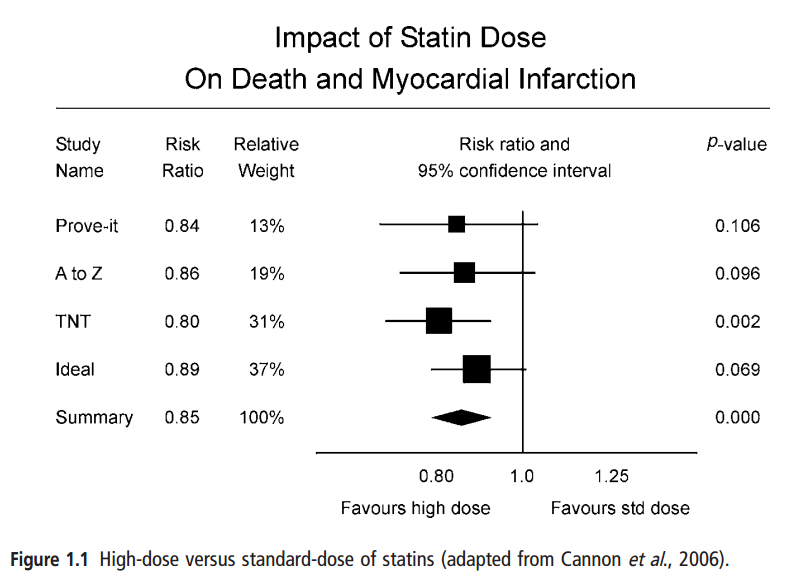
\includegraphics[scale=0.5]{chunks/cannonetal2006}
\par\end{centering}
\caption{\label{fig:A-forest-plot}A \emph{forest plot} of the studies included
in \cite{cannon_meta-analysis_2006} meta-analysis on statins. The
table is from \cite[p. 4]{Borenstein2011-yx}.}
\end{figure}
Despite being terribly important, often the difference between life
and death\footnote{See the preface of \cite{Borenstein2011-yx} for a story
of how earlier adoption of meta-analyses could have saved the lives
of thousands of babies that suffered from sudden infant death syndrome.}, meta-analyses have two weaknesses. The first weakness is subjectivity.
For while a meta-analysis is by nature less subjective than a narrative
review, it might still be too subjective to settle a scientific question
once and for all. This problem is emphasized by \cite{Stegenga2011-zo},
and is exemplified by the continuing meta-analysis wars in the research
on the effect of violent video games on aggressive behavior, as discussed
by \cite{elson_twenty-five_2014}. The other weakness are systematic
biases that are hard to model. One of these biases is \emph{publication
bias}, the tendency to publish only positive results. The other is
\emph{p}-hacking, the phenomenon where researchers unconsciously manipulate
studies to get small \emph{p}-values.

\subsection{The problems of meta-analysis}

There is a certain degree of subjectivity in any data analysis, and
the greater leeway to make subjective choices, the stronger the tendency
for the authors to make self-serving choices. An extreme variant of
this is covered by \cite{Steegen2016-fj}, where it was
shown that a study about the combined effect of relationship status
and fertility could be analyzed in at least 210 different ways. Only
some of these gave results in the desired direction and, not surprisingly,
the published paper had results in the desired direction as well. 

The meta-analyst must choose which studies to include in her meta-analysis.
There is often a good deal of subjectivity here, for it is rarely
so that a study is unambiguously eligible for inclusion. There are
many reasons to exclude a potential study from a meta-analysis. An
oft-discussed bias is \emph{location bias}. If the meta-analysts
are English, they will have a hard time incorporating foreign language
studies into their meta-analysis \parencite{Egger1998-kj}, resulting
in a location-specific meta-analysis. In addition, the meta-analyst
will often include only studies from peer-reviewed scientific journals,
ignoring studies from dissertations or the gray literature. There
are trade-offs involved in the choice of including non-published studies.
On one hand, inclusion of unpublished studies might reduce publication
bias \parencite{Egger1997-ue},
but it could also increase the bias of the meta-analysis. The reason
is that the meta-analyst must rely on her network of researchers to
obtain the unpublished studies -- but her network is likely to be
biased in exactly the same direction as she is. An example of this
effect is found in \cite{Ferguson2010-to}'s discussion of \cite{Anderson2010-ki}'s
meta-analysis on the effect of violent video games on behaviour. The
literature on video game violence and aggression is divided into two
camps. The camp associated with Anderson holds that violent video
games cause aggression, the camp associated with Ferguson holds that
they do not. In order for a meta-analysis to be accepted by all camps,
it should not be biased against including studies from the opposite
camp. However, \cite{Anderson2010-ki} included several unpublished
studies in their meta-analysis, but all were from their own Anderson's
group or associated groups.
\begin{quote}
For example, of two unpublished studies, both are from Anderson et
al.'s broader research group. Of three in-press manuscripts
included, two (67\%) are from the Anderson et al. group. Of conference
presentations included, 9 of 12 (75\%) are from the Anderson et al.
group and colleagues. 
\begin{flushright}
-- \cite[p. 2]{Ferguson2010-to}
\par\end{flushright}

\end{quote}
Another source of subjectivity is whether to only include randomized
controlled trials. There is broad agreement that only randomized controlled
trials should be included in a meta-analysis if these trials exists
\parencite{Egger1997-ue}. The reason is that randomized
controlled trials are not affected by confounders in the same ways
as e.g. case control studies and other observational studies. However,
excluding observational studies violates the principle of total evidence,
that your conclusions should be based on all available evidence, not
just a subset of it, see \cite{Stegenga2011-zo} for an extended
discussion.

A reason to exclude a study is that it does not fulfill a list of
best practices. Not all studies are created equal, some are simply
of better quality than others. For instance, a subset of studies might
have much better measuring instruments than the rest, making it reasonable
to include only the studies with the good measuring instrument. But
this is yet another source of subjectivity. As an example \parencite[taken from][p. 6]{lakens_reproducibility_2016},
consider the following ``best-practice'' from \cite{Anderson2010-ki}'s
aforementioned meta-analysis on the effect of violent video games
on behaviour. In order to qualify for a best-practice study, the control
group must be exposed to a non-violent game, while the treatment group
must be exposed to a violent game. One unaccepted treatment-control
pair was \emph{Mortal Kombat} vs \emph{Sonic the Hedgehog.} While
Mortal Kombat is a fighting game infamous for its violence, Sonic
the Hedgehog involves playing a hedgehog jumping on robots, and would
easily be classified as among the least violent games by many researchers.
On the other hand, an accepted treatment-control pair was \emph{Simpsons
Hit \& Run }vs \emph{Grand Theft Auto 3, }even though Simpsons Hit
\& Run involves pulling people out of their car in high-speed situations. 

Finally, studies can be excluded since they look suspicious. There
are many cases of both reporting errors \parencite{nuijten_prevalence_2016}
and downright fraud in the research literature, with Diedrik Stapel
being a high-profile fraudster from social psychology. Since research
data is seldom available, the meta-analyst will not be able to check
the veracity of the reported results in each research paper. This
can lead to exclusion of studies on seemingly ad-hoc grounds. As an
example, take \citeauthor{ferguson_angry_2015}'s 2015 meta-analysis
on the effect of violent video games on aggressive behaviour. In this
analysis, he excluded the study of \cite{gentile_effects_2009} due
to what \cite{ferguson_angry_2015} called ``bouncing beta'' regression
coefficients, or regression coefficients of equal magnitude going
in opposite directions. For a response to this claim, see \cite{gentile_what_2015}'s
rejoinder.

\subsubsection{Choice of statistical technique}

After the meta-analyst is done collecting her data, she must chose
how to analyze them. Now she is faced with two categories of models,
namely the class of \emph{fixed effect models} and \emph{random effects
models} \parencite[chapter 10]{Borenstein2011-yx}. In order
to explain these models, I will need some technical notation. So let
$N(\mu,\sigma)$ denote the normal distribution with mean $\mu$ and
variance $\sigma^{2}$, and allow $z_{i}$ to be the estimated effect
size of the $i$th study. Under this simple set up, the fixed effects
model works under the assumption $z_{i}\sim N(\mu,\sigma_{i}n_{i}^{-1/2})$.
The pith of this model is that all studies are assumed to \emph{exactly
equal}. On the face of it, this is an unacceptably unrealistic assumption.
Still, the model will often be the best choice, mostly due to the\emph{
bias-variance trade-off} \parencite[p. 37]{friedman_elements_2001}. Since
our data is imprecise, it is always possible to get our estimates
horribly wrong. When we have many parameters in comparison to the
data size, the possibility of this happening goes from possible to
probable. The consequence is that a model with many parameters will
increase the variance of our estimates. On the other hand, a model
with few parameters will not give us the correct information even
with \emph{infinitely much data} -- there is an inherent bias in
the model. In conclusion, there are good reasons to believe fixed
effects models should perform well even though they are simple. Other
reasons to prefer fixed effects models is their interpretability.
They reflect what researcher hopes for an effect to be: A reliable,
consistent phenomenon. 

On the other hand, studies are always slightly different, also in
unobservable ways, and this difference is called study \emph{heterogeneity}.
This heterogeneity is captured by the normal distribution $N\left(\mu,\tau^{2}\right)$
above. In essence, we assume that all the heterogeneity can be accounted
for by a normal distribution. Examples of heterogeneity includes ``\emph{diversity
in doses, lengths of follow up, study quality, and inclusion criteria
for participants.} \parencite{higgins_measuring_2003}`` The models used
to capture this between-study variance are the random effect models.
In symbols, the linear random effect model is

\begin{eqnarray}
\mu_{i} & \sim & N(\mu_{0},\tau).\label{eq:Random effects}\\
z_{i} & \sim & N(\mu_{i},\sigma_{i}n_{i}^{-1/2})\nonumber 
\end{eqnarray}

There are more choices to be made regarding data analysis. Both main
classes of models can be estimated using a wealth of different methods,
both frequentist and Bayesian. A good case for Bayesian analysis can
be made on the grounds of \emph{regularization} (see e.g. \cite{simpson_penalising_2017}).
Pure maximum likelihood is unstable, making it possible to obtain
far too large estimates when the sample size is small. On the other
hand, a Bayesian approach requires a prior, which adds yet another
layer of subjectivity. Moreover, if random effects are used, the meta-analyst
must decide whether she wants to use the normal distribution or something
else to model it. Still, the most important decision concerns which
covariates be included. By adding information about e.g. age of participants,
the length of the study, or the type of intervention used, the conclusions
of the meta-analysis can change dramatically.

Some academic fields will have more heterogeneous studies than others.
One example of a heterogeneous field is \emph{social priming} research,
where the exact experiments are significantly changed from study to
study since the effects studied are assumed to be sensitive to the
minutiae of the experimental conditions. Since random effects models
incorporates differences among studies, using a random effects model
looks like a no-brainer in this subfield of psychology. \cite{oyserman_does_2008}
is a highly cited meta-analysis of collectivism vs individuals primes,
with over $900$ Google scholar citations. Still, \cite{lakens_reproducibility_2016}
claim that \cite{oyserman_does_2008} uses the wrong model, namely
fixed effects instead of random effects. While \citeauthor{oyserman_does_2008}
obtain a statistically significant effect size in their original meta-analysis,
\cite{lakens_reproducibility_2016} do not obtain significance in
their reanalysis with a random effects model. But recall the remark
above about the virtues of fixed effects models -- their estimates
might be less accurate, but are more precise. The researchers belong
to two different sides in an ongoing debate about the existence of
social priming effects, and both can justify their choice of model
if need be.

\subsubsection{Publication bias and $p$-hacking}

In 1959, \citeauthor{Sterling1959-cq} noted that many journals
in psychology operated with strict understanding of statistical significance
-- a result was reported as statistically significant if its associated
$p$-value was less than $0.05$. Then he hypothesized that this rigid
rule would cause that studies with non-significant results not to
be published. In order to test this hypothesis, he sampled $364$
papers from four psychology journals and registered the results from
the statistical tests contained in them. The result was staggering:
Out of $296$ significance tests, only $8$ were non-significant at
the $0.05$ level. To account for such an observation without invoking
publication bias would require extraordinary assumptions on the ability
of psychologists to find real effects. The phenomenon that almost
only publications with a $p$-value less than $0.05$ are published
is commonly referred to as \emph{publication bias} or the \emph{file-drawer
problem \parencite{rosenthal_file_1979}}

While the most famous cause of publication bias is the tendency for
scientific journals to only accept articles containing statistically
significant results, typically at the level of $0.05$ \parencite{simmons_false-positive_2011},
it should be understood more broadly. In this article, publication
bias refers to the tendency to not publish null-results, or even weak
results. The exact mechanism behind publication bias are unknown.
For instance, a study reaching ``borderline statistical significance''
or even ``trending towards significance'', with a $p$-value at
say $0.07$, is probably more likely to be published than a study
with a $p$-value of $0.23$. If there is evidence for null-effect,
the paper is more likely to be published when the evidence for the
null effect is strong, which is the case with large $n$ studies. 

A cousin of publication bias is\emph{ $p$-hacking}, the process of
actively changing the data analysis in order to obtain significant
results:
\begin{quote}
While collecting and analyzing data, researchers have many decisions
to make, including whether to collect more data, which outliers to
exclude, which measure(s) to analyze, which covariates to use, and
so on. If these decisions are not made in advance but rather are made
as the data are being analyzed, then researchers may make them in
ways that self-servingly increase their odds of publishing. 
\begin{flushright}
-- \cite[p. 1]{simonsohn_p-curve:_2014}
\par\end{flushright}

\end{quote}
As emphasized by \cite{simonsohn_p-curve:_2014}, the presence of
$p$-hacking creates publication bias even when \emph{all} conducted
studies are published. In fields such as social psychology, where
there is no consensus about how to measure different constructs, which
statistical methods to use, or what variables your can condition on,
it is almost always possible to get statistically significant result
out of your study\footnote{See \cite[p. 2, study 2]{simmons_false-positive_2011} for a humorous
instance of this, where a literally impossible phenomenon is established
with $p<0.05$.} It is even possible to obtain enough results to fill four papers
with spurious results, as was the case with food scientist Brian Wasnink,
see \cite{van_der_zee_statistical_2017} for a discussion of Wasnink
four papers on pizza buffets. This newfound focus on $p$-hacking
changes how we view publication bias -- for instance, the common-sense
claim that ``\emph{when a pattern is seen repeatedly in a field,
the association is probably real, even if its exact extent can be
debated}\textquotedblright{} (\cite{ioannidis_why_2008},cited from
\cite{simonsohn_p-curve:_2014}) is likely to be incorrect. Since
$p$-hacking is ubiquitous, it is the \emph{popularity }of a purpoted
effect which determines the number of published studies on the same
or similar effects, not the likelihood of obtaining a significant
result.

Publication bias and \emph{p}-hacking are ubiquitous in psychology.
A solid piece of evidence for this claim is the study of \cite{Motyl2017-dx}.
They collected all critical effect size estimates and \emph{p}-values
from the four top-tier journals \emph{Journal of Personality and Social
Psychology}, \emph{Personality and Social Psychology Bulletin}, \emph{Journal
of Experimental Social Psychology}, and \emph{Psychological Science}.
A critical effect size or \emph{p}-value is one that is used to support
the core hypothesis of the paper. That is, the list of statistics
does not include statistics associated with auxiliary questions such
as ``are there significantly more woman than men in the sample''.
These statistics were collected over the pre-replication crisis year
$2003$--$2004$ and the post-repliacation crisis years $2013$--$2014$. 

Figure \ref{fig:motyl} plots estimated effect sizes from \cite{Motyl2017-dx}
together with the line $y=1.96/\sqrt{n}$, the treshold for significance
using the two-sided normal \emph{p}-value. The random effects meta-analysis
model of equation (\ref{eq:Random effects}) yields the estimates
$\hat{\mu}_{0}=0.42$ and $\hat{\tau}_{0}=0.34$, Notice how the studies
cluster just about treshold for significance, which is extremely unlikely
under normal sampling.

\begin{figure}
\noindent \begin{centering}
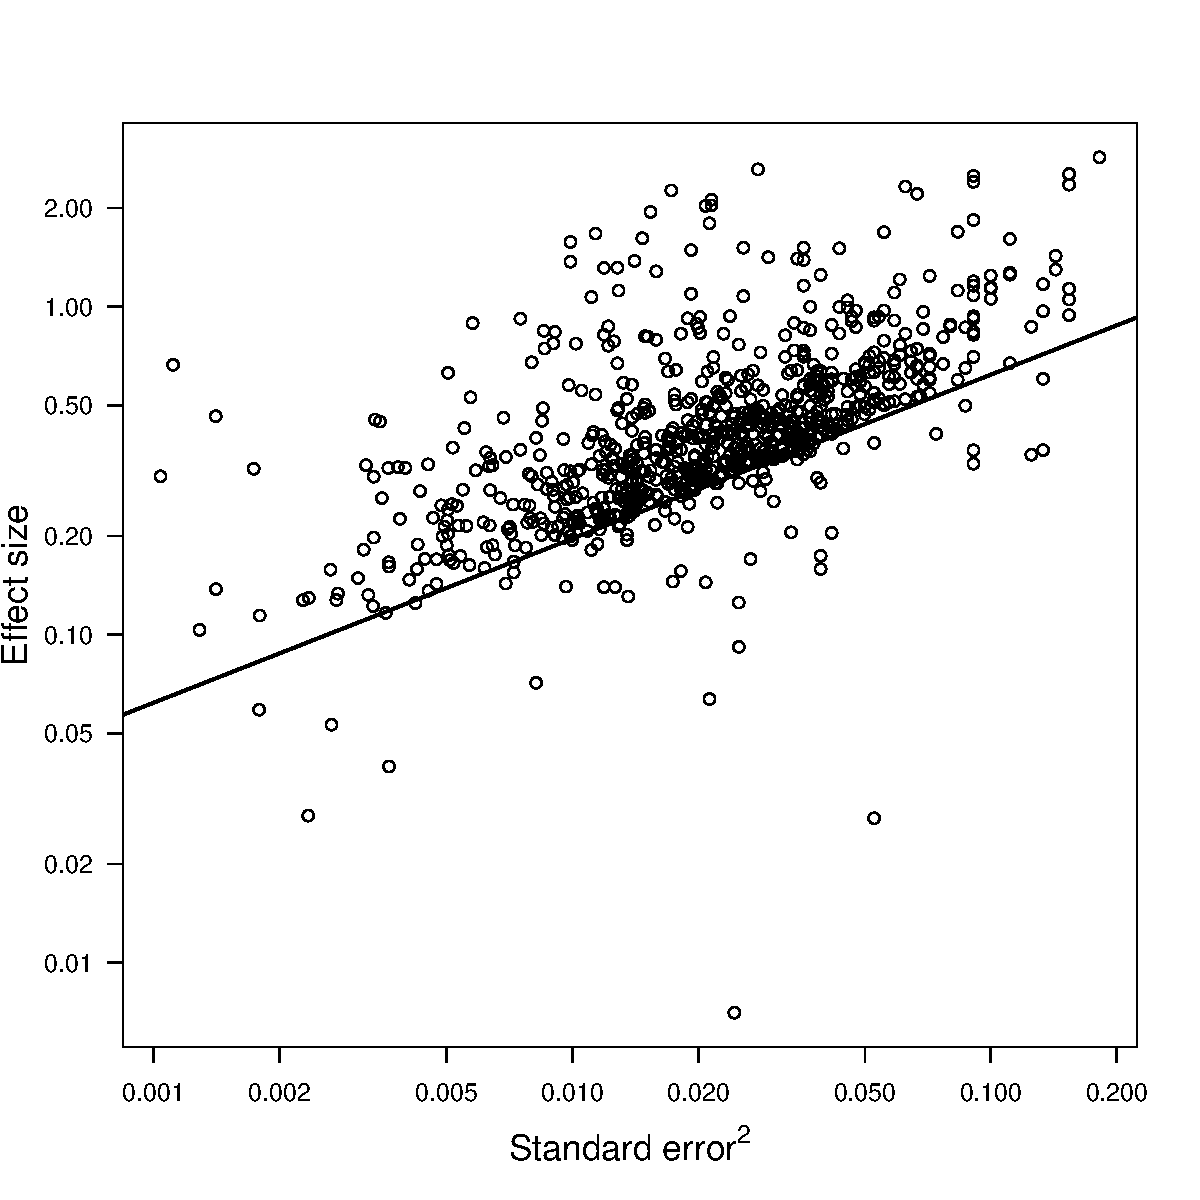
\includegraphics[scale=0.5]{chunks/motyl}
\par\end{centering}
\caption{\label{fig:motyl}Estimated effect sizes and squared standard errors
from \cite{Motyl2017-dx}. The black line is $y=1.96/\sqrt{n}$,
the treshold for significance using the two-sided normal \emph{p}-value.
Both axes are logarithmic. The number of studies is $n=862$, and
the percentage significant results is $91.5\%$.}
\end{figure}


\subsubsection{Correction for publication bias and $p$-hacking}

There are several methods that attempts to identify and even correct
for publication bias. The most widely used is the \emph{funnel plot}
of \cite{Egger1998-kj}, where the standard error of each study
is plotted against its effect size. Under severe publication bias,
this plot will be skewed. This is because small studies, which will
typically be those with high standard errors, must have large estimated
effect sizes in order to cross the $p=0.05$ boundary. An example
of such a plot is found in figure 2.1.

\begin{figure}
\noindent \begin{centering}
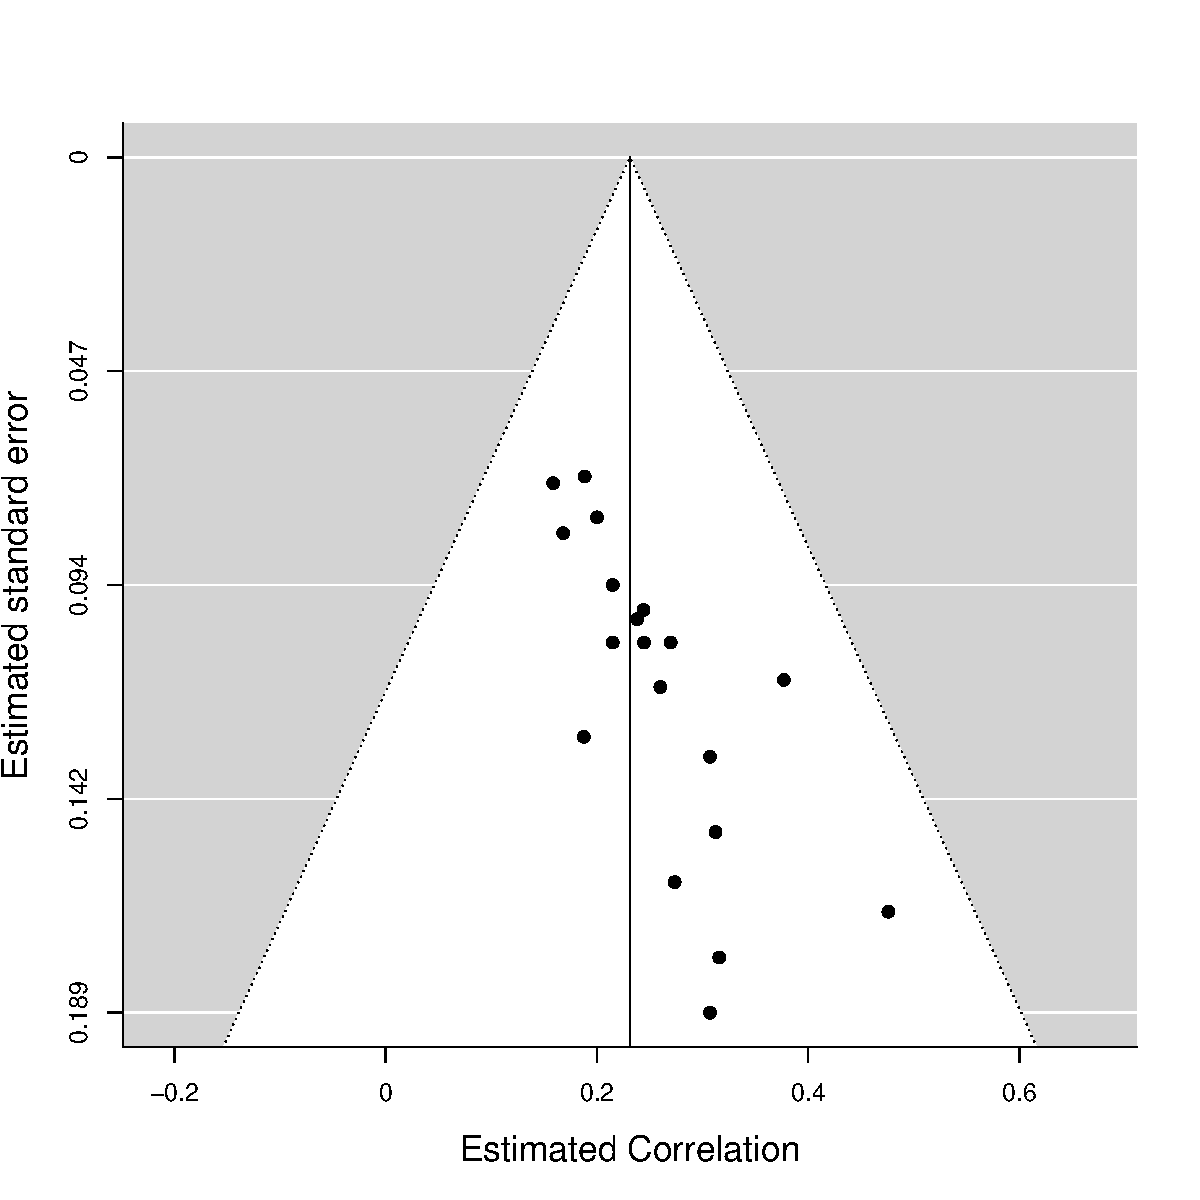
\includegraphics[scale=0.5]{chunks/anderson}
\par\end{centering}
\caption{\label{fig:A-funnel-plot}A funnel plot of a subset from the meta-analysis
of \cite{Anderson2010-ki} on the effect of violent video games
on aggressive behavior. The funnel plot is highly skewed to the left,
which indicates severe publication bias. The funnel plot was made
with the $\mathtt{R}$-package \cite{team_r_2000}
$\mathtt{metafor}$ \parencite{viechtbauer_conducting_2010}.}
\end{figure}

Under severe publication bias, this plot will be skewed. Building
on this method intuition, the authors propose to estimate a publication
bias-corrected effect size by running the regression
\[
z_{i}\sim\theta+\beta\widehat{s}_{i}+\epsilon_{i},
\]
where $\theta$ is the adjusted effect size and $\beta\neq0$ indicates
the presence publication bias This method is called PET \parencite{stanley_beyond_2005}.
But PET is not the only regression-based method for publication bias
correction. Another popular method is PET-PEESE \parencite{Stanley2014-gx},
a modified version of the above, applied mostly in economics research
and recently to psychology \parencite{carter_series_2015}. This method
is not without critics. \cite{gervais_putting_2015} claims the method
systematically underestimates the effect size in presence of publication
bias, making almost any effect appear to be indistinguishable from
$0$. In addition, \cite{simonsohn_[59]_2017} runs simulations to
show that the method fails in presence of inter-study heterogeneity.
The most popular method in medicine is named trim and fill \parencite{Duval2000-ct},
which is based on removing and adding non-observed studies to the
funnel plot in order to make it symmetric. The $p$-curve of \cite{simonsohn_p-curve:_2014}
has proven popular in psychology. This method is based on the theoretical
shape (under the null of no $p$-hacking) of the probability density
function obtained from the $p$-values from a set of studies. For
a simulation study comparing methods to account for publication bias,
see \cite{moreno_assessment_2009}.

All these methods share a serious shortcoming. Popular statistical
methods, such as linear regression and logistic regression, are based
on\emph{ explicitly defined models}. These models allows for clear
cut estimation of parameters, parameters with univocal definitions
and interpretations. The methods for publication bias are not based
on explicit models. As such, their estimated quantities are hard to
interpret, and are defined in an offhand way. For instance, PET-PEESE
is based on one half intuition, one half semi-rigorous mathematics;
the $p$-curve of is based on statistical properties of a null-model
we assume that is false. While there are several statistical methods
used to model heterogeneity, as discussed in the previous chapter,
none of them have been directly extended to take publication bias.
The product of this flaw is that all corrections for publication bias
are \emph{ad hoc}, which partially explain their poor performance. 

The meta-analyst will have to make a choice of correcting for publication
bias or not. If she opts to correct for publication bias, she is faced
with a large number of different methods, none of them particularly
good, but if her choice is no, her resulting estimates might be severely
biased. The effect of this choice is potentially tremendous. As an
illustration, I take a well-known contentious issue from economics:
What is the relationship between the minimum wage and employment?
The predictions from economic theory about this are unequivocal: Rising
the minimum wage should raise the rate of unemployment. There are
two reasons why: First, when the minimum wage is raised above the
competitive wage, the employer will shift his spending towards other
venues such as capital investments. Second, the industries affected
will increase their prices to consumers, reducing the demand for labor
in turn. \cite{doucouliagos_publication_2009} studies the empirical
research the relationship between a minimum wage floor and employment.
Their meta-analysis contains $64$ studies, which in turn contain
a total of $1474$ employment elasticity estimates. The average elasticity
was $-0.19$, while the fixed effects meta-analytic estimate was $-0.054$,
both highly significant. However, their publication bias-corrected
estimate was the meager $-0.01$. In the words of \cite{doucouliagos_publication_2009}:
``An elasticity of -0.01 has no meaningful policy implications. If
correct, the minimum wage could be doubled and cause only a 1 per
cent decrease in teenage employment.'' In this case the decision
to correct for publication bias reduced the effect size estimate with
a factor of $5$. Needless to say, this could have huge policy implication,
recall the recent push towards rising the minimum wage in California
and other U.S. states.

Since publication bias and $p$-hacking is ubiquitous and its effect
can make the difference between two radically different conclusions,
good methods for dealing with it is needed. Since the current methods
do not live up to the task, research on improving these methods are
needed. Even more important, scientist should rigorous in their usage
of methods designed to avoid publication bias and $p$-hacking, for
instance study pre-registration. 

\subsection{Back-of-the-envelope calculations }

A large part the daily lives of researchers is spent in reading and
critically engaging with other peoples research. Prior to the replication
crisis, a common way to judge the worth of an effect was to look at
its \emph{p}-value or \emph{t-}value. If the \emph{p}-value was smaller
than $0.05$, or the \emph{t-}value larger than approximately $2$,
results looked impressive enough to be worthy of consideration. While
plenty of researchers believe this way to do consume research is bad
\parencite{Gigerenzer2004-oc}, it is not without its mertis. We have
limited attention span and need to abide by some decision rules; what
we need are justified decision rules that will not lead us astray
with an unacceptably high probability.

Making some half-plausible assumptions, there is simple a way to correct
effect sizes for publication bias and \emph{p}-hacking. This back-of-the-envelope
method is based on a simple model of selection for significance, where
we observe only significant normal $X$s. Assume $X\sim N(\mu,n^{-1/2})$
and let $U=\Phi(-n^{1/2}X)$ be the standard one-sided $p$-value.
The expectation of the left-truncated normal is \parencite[Section 10.1]{Johnson1994-ag}

\begin{equation}
\mu+\sigma M'\left(\frac{a-\mu}{\sigma}\right).\label{eq:mean of truncated normal}
\end{equation}
In our case, $a=c_{\alpha}n^{-1/2}$ and $\sigma=n^{-1/2},$ and the
expectation equals $\mu+n^{-1/2}M'(c_{\alpha}-n^{1/2}\mu)$. When
$\mu=0$ and $\alpha=0.05$, get $E(X\mid n^{1/2}X>c_{\alpha})=n^{-1/2}\alpha^{-1}\phi(c_{\alpha})\approx2n^{-1/2}.$
This value is easy to remember and compute, and provides a realistic
baseline to compare effect sizes against. In a world free of biases,
we would informally compare an effect size against $0$. In a world
with publication bias and \emph{p}-hacking, comparing against $2n^{-1/2}$
smarter and almost as easy. From the data set of \cite{Motyl2017-dx}
we just looked at, we get $2\overline{n^{-1/2}}=0.24$. That is, we
would expect a mean effect size of $0.24$ from psychology even when
the true mean is $0$, assuming complete selection for significance
and the validity of the normal approximation. The actual mean of the
data set, $\overline{\theta}=0.45$, does not look that impressive
anymore.

There are strong reasons to care not only about \emph{p}-values, but
also about effect sizes \parencite{Funder2019-tg}. The natural way to
estimate $\mu$ is to use the maximum likelihood estimator $\hat{\mu}$.
While this quantity is easy to calculate numerically, it is hardly
convenient to use when reading a paper. Luckily, there are simple
bounds for the maximum likelihood estimator.
\begin{proposition}
\label{prop:maximum likelihood bounds}The maximum likelihood estimator
of $d$, called $\hat{d}$, based on a single observation $x$ from
a study with $n$ participants is bounded by 
\[
l(x)\leq\hat{d}(x)\leq u(x).
\]
The bounds are equal to
\begin{eqnarray}
l(x) & = & x-\frac{1}{n^{1/2}\delta},\label{eq:lower bound}\\
u(x) & = & x-\frac{1}{n^{1/2}\delta}\max\{1-\delta^{2},0\}.\label{eq:upper bound}
\end{eqnarray}
where $\delta=n^{1/2}x-\Phi^{-1}(1-\alpha)$.
\end{proposition}
Proposition \pageref{prop:maximum likelihood bounds} is a straight-forward
corollary of the following propositon. 
\begin{proposition}
\label{prop:ml bouds}Let $X_{1},\ldots,X_{N}$ be independent samples
from a left-truncated normal. Assuming known truncation point $a$
and standard deviation $\sigma$, the maximum likelihood estimator
$\hat{\mu}$ of $\mu$ is bounded by
\begin{equation}
\overline{x}-\frac{\sigma^{2}}{\overline{x}-a}<\hat{\mu}<\overline{x}-\max\left(\frac{\sigma^{2}}{\overline{x}-a}-(\overline{x}-a),0\right).\label{eq:ml bounds}
\end{equation}
\end{proposition}
\begin{proof}
Differentiating the logarithm of the density of a truncated normal,
we find that the maximum likelihood estimator is the solution to $\mu=\overline{x}-\sigma M'([a-\mu]/\sigma),$where
$M'(\text{\ensuremath{\theta}})=\phi(\text{\ensuremath{\theta}})/\Phi(-\text{\ensuremath{\theta}})$
is the inverse Mills' ratio. The inverse Mills' ratio can be bounded
elementary functions \parencite{Yang2015-pa}. In particular, it can be
bounded by \parencite[Equation 32]{Gasull2014-hn}
\begin{equation}
M_{u}(\theta)=\frac{1}{2}(\sqrt{\text{\ensuremath{\theta}}^{2}+4}+\text{\ensuremath{\theta}})>M'(\text{\ensuremath{\theta}}),\label{eq:Mills' ratio inequality}
\end{equation}
and 
\begin{equation}
M'(\text{\ensuremath{\theta}})>\frac{1}{4}(\sqrt{\text{\ensuremath{\theta}}^{2}+8}+3\text{\ensuremath{\theta}})=M_{l}(\theta)>\theta.\label{eq:Mill's ratio inequality (2)}
\end{equation}
The functions $M(\text{\ensuremath{\theta}})$ in these inequalities
are increasing in $\text{\ensuremath{\theta}}$, hence $\overline{x}-\sigma M([a-\mu]/\sigma)$
is icreasing in $\mu$. Assume $\mu_{u}$ satisfies $\mu_{u}=\overline{x}-\sigma M_{u}([a-\mu_{u}]/\sigma)$.
Since $M_{u}(\theta)>M'(\theta)$, we have $\overline{x}-\sigma M'([a-\mu_{u}]/\sigma)<0$
too, thus $\mu_{u}<\hat{\mu}$. Likewise, if $\mu_{l}$ satisfies
$\mu_{l}=\overline{x}-\sigma M_{l}([a-\mu_{l}]/\sigma)$, then $\mu_{l}>\hat{\mu}$.
Now define $l(\overline{x})=\mu_{u}$ and $u(\overline{x})=\mu_{l}$.
Now, to find $l(\overline{x})$, solve
\[
\mu=\overline{x}-\sigma\frac{1}{2}(\sqrt{\text{\ensuremath{([a-\mu]/\sigma)}}^{2}+4}+\text{\ensuremath{[a-\mu]/\sigma}})
\]
to get $\mu=\overline{x}-\sigma^{2}/(\overline{x}-a)$. The upper
bound $u(\overline{x})$ can be found in the same manner, using both
the lower bounds $M_{l}(\theta)$ and $\theta$ and choosing the best
option.
\end{proof}
    \section{Open science with \texttt{R}}

\texttt{R} is not only a popular language among statisticians. Its popular among other scientists as well, social scientists and biologists in particular. The \texttt{R} community is brimming with dedicated user, with roughly $16,000$ \texttt{CRAN} packages as of August 2020. The large user-base and design of the language makes it the ideal language for statistics, with Python being the only rival. \texttt{R} has a sizable user base. For example, there are at least 16 packages dedicated to univariate density estimation \parencite{Deng2011-bk} and at least 14 implementations of isotonic regression \parencite{Busing2019-tv}. 

\texttt{R} packages are accessible and often easy to use, which makes it possible for other people to find errors and correct your mistakes. If you multiply by $2$ instead of $\sqrt{2}$ and don't make the code public, you will never know. Most methods development is exploratory, and works by carefully experimenting with different setups, starting with the well-known then slowly proceeding to the more difficult. High-quality \texttt{R} packages helps your colleagues do their research, since they can build, incrementally, on your trusted work.  

You can trust mathematical results to the extent you and your colleagues can verify the proofs. Importantly, a good proof should be relatively cheap to verify in terms of time and effort. This is a strong incentive for writing correct proofs. Simulations, however, are usually a chore to write and to verify. We only do them because we have to. Probably no one will try to replicate them. To make simulations, custom Markov chain Monte Carlo samplers, and similar difficult programs worth considering seriously, the code should be both documented, tested, and open. For why should be expect statisticians to behave better than psychologists?

Sharing code can make a difference even when using the best-known methods. \textcite{McCullough2003-zd} discusses how the coefficients of a Probit regression couldn't be reproduced. In their, case the irreproducibility occurred since the likelihood didn't have a maximum, but the numerical algorithm failed to inform the user that a maximum wasn't found. The authors go on to describe how one can, through force of labour, verify or disconfirm that a proposed maximum is in fact a maximum. Considering that many, if not the majority, of research statisticians are not specialists in numerical analysis, it is irrational to expect every statistician to write perfect numerical solvers for every maximization problem he studies. Since sharing well-documented code makes it much easier for researchers to scrutinize your work, problems such as non-sensical estimates are far more likely to be uncovered.

In the Transparency and Openness Promotion guidelines \parencite{Nosek2015-hh}, the highest level of analytical openness states that ``Code must be posted to a trusted repository, and reported analyses will be reproduced independently before publication.''. At the time of writing, 26 journals adhered to this code according to https://topfactor.org/. Such strong codes were even enforced by some journals years ago according to \textcite{Nosek2015-hh}, who states that ``the journals Political Analysis and Quarterly Journal of Political Science require authors to provide their code for review, and editors reproduce the reported analyses publication. ``

How does statistical journals compare? I checked the instructions to authors pages of seven top journals to find out. \emph{Biometrika} encourages authors to provide code and data, but does not require it, as ``Biometrika strongly encourages authors to make all data and software code on which the conclusions of the paper rely available to readers.'' The Journal of the American Statistical Society, similarly,``[...] strongly encourages all authors to submit datasets, code, other programs, and/or extended appendices that are directly relevant to their submitted articles, [...].'' \emph{Journal of the Royal Statistical Society, Series B}, has a slightly less ambiguous statement, namely that ``it is the policy of the Journal of the Royal Statistical Society that published papers should, where possible, be accompanied by the data and computer code used in the analysis. Both data and code must be clearly and precisely documented, in enough detail that it is possible to replicate all results in the final version of the paper.'' The Journal of Graphical and Computational Statistics has the strongest demand, stating that ``Authors are expected to submit code and datasets as online supplements to the manuscript. Exceptions for reasons of security or confidentiality may be granted by the Editor.`` The journals \emph{Annals of Statistics}, \emph{Electronic Journal of Statistics}, and \emph{Bayesian Analysis} say nothing about code and data in their instructions to authors pages.

Creating high-quality \texttt{R} packages is made easy by the multitude of aids conferred by the \texttt{R} ecosystem. A high-quality \texttt{R} package should consist of high-quality code. It should be well-documented, be tested, conform to the standards of the \texttt{R} community, such as passing the \texttt{CRAN} incoming checks and having vignettes.

Code quality is an elusive concept not everyone agrees on what it is. \textcite[Section 1.1.2]{Spinellis2006-dd} analyses code quality as an amalgamation of six desirable features of code: Functionality, reliability, usability, efficiency, maintainability, and
portability. Let us take a closer look at usabilityand maintainability.

A package is usable if its external interface is easy to understand, easy to learn, and easy to use. When making a package implementing a new kind of regression, for instance with \textit{t}-distributed errors, it will be much easier to use if it follows the patterns of the \texttt{lm} function with associated generics such as \texttt{predict} and \texttt{summary} than if it follows an entirely new convention. Usability concerns the complexity of the argument list and limiting the number of jobs one function can take on. Moreover, the scope of packages should preferably be limited. If the main feature of a package is isotonic regression, your novel \texttt{print} method for \texttt{ANOVA} objects should probably be left out.

Code is maintainable when it is easy to understand, extend, and modify the code without breaking functionality and introducing bugs. Maintainable code involves reusing existing code, especially code from base \texttt{R}, making the code modular, and writing compact code with limited complexity.  In most projects it is desirable for the code to follow the same style. One of the most famous \texttt{R} styles is the \texttt{tidyverse} style \parencite{Wickham_undated-sw} and Google's \texttt{R} style \parencite{noauthor_undated-pk}. 
Much \texttt{R} package development takes place on Github and other Git-based platforms such as Gitlab. These platforms allow for version control, code sharing, collaboration, and issue tracking. Lately, it has become popular to use Git to collaborate on papers too, often with \texttt{R} taking the center spot.

There are tools that greatly simplify the production of high-quality \texttt{R} code. Some of the most important are \texttt{devtools} \parencite{devtools}, for creating and disseminating \texttt{R} packages, and \texttt{roxygen2} \parencite{roxygen2} for automatized creation of documentation. The packages \texttt{knitr} \parencite{Xie2014} and \texttt{R} markdown allows you to create manuscripts, blog posts, \texttt{R} package vignettes, reports, and even Beamer presentations without leaving \texttt{R}.

Documentation allows the user to use the software without guessing what it does. Ideally, the user will understand what your code does without having to read your code at all. And in this sense, high-quality documentation lowers the bar for both users and contributors to engage with your code and understand your research. Documentation forces you think about how general your function is, what its input should be, and as a consequence, what it can be used for. As a consequence, documentation leads to better code. When you revisit your code $4$ years from now, you can actually read it and understand what it does. 

An essential part of a high-quality coding project are \emph{formal tests}, or tests that are purposefully designed to make sure your code does what it should. Formal testing of code has plenty of benefits. First and foremost, testing increases the quality of your code. According to \textcite[Chapter 7]{Wickham2015-ik}, testing causes bugs to disappear, better code structure, and more robust code. An \texttt{R} package with plenty of formal tests can be trusted more than one without tests. That tests have been written and passed demonstrates the program does at least something correctly, provided the tests are well-written. Second, tests inspire confidence in the authors. An author who carefully writes tests is less sloppy that one who cannot find the time to or does not bother. Third, since tests make code better, the code can be trusted to work well too. An especially good practice for \texttt{R} packages is to cross-check the output of functions. For instance, the \texttt{R} time series package \texttt{memochange} \parencite{memochange} checks the output of every function against outputs in the literature.

Publishing in the Journal of Open Source Software is an accessible way to get credit for your work in creating \texttt{R} packages. The journal is solely focused high-quality software, including solid documentation and tests, and the paper itself is not at the centre stage. Developers are allowed to spend time on what they do best and what is meaningful in software development, not waste time in adhering to arbitrary journal style requirements and writing barely-read literature reviews. Most papers in the Journal of Open Source Software are between one and two pages long, and could potentially be written in an hour or less. 
    
\section{Psychometrics}
In the animated 1937 classic \textit{Clock Cleaners}, Mickey Mouse, Donald Duck, and Goofy are working as janitors in a clock tower. As usual, Goofy is dimwitted and carefree, Donald Duck gets fits of anger, and Mickey Mouse is kind and compassionate. Goofy mistakes a statue for a lady, Donald Duck throws a temper tantrum at a spring, and Mickey Mouse does everything he can to save Goofy from falling to certain death. This is not the only animated movie were these characters behave like this. Donald Duck's fiery temper -- and bad luck -- is what he's known for, and something you'd expect to see in any movie featuring him. Likewise, Goofy is always thickheaded. We say that these characters have \textit{stable psychological traits}. And real humans have them too. There are people you would describe as temperamental. In almost every situation, they are more prone to getting angry than others.

Psychometrics is about the study and quantification of psychological traits such as temperament. These traits cannot be directly measured though. Even if you think every individual has, in Platonic sense, a real variable $Z$ called "temperament", you would not be able to measure it directly. For these traits are not observable, they are \textit{latent}. Instead of observing $Z$ directly, we observe a random vector $X$ of proxies for $Z$. In most cases these proxies are responses to a questionnaire, usually on \emph{Likert items}. A Likert item is the response to a question with ordered alternatives ranging from e.g. strongly disagree to strongly agree. Table \ref{tab:IPIP} shows five questions from the International Personality Item Pool \parencite{Goldberg1992-hp}, all of them supposedly related to the trait \textit{agreeableness}.

\begin{table}
\caption{\label{tab:IPIP}Five questions loading on \textit{agreeableness} from the International Personality Item Pool}
\noindent \begin{centering}
\begin{tabular}{lccccc}
 & $1$ & $2$ & $3$ & $4$ & $5$\tabularnewline
Am indifferent to the feelings of others.  & $\bigcirc$ & $\bigcirc$ & $\bigcirc$ & $\bigcirc$ & $\bigcirc$\tabularnewline
Inquire about others' well-being. & $\bigcirc$ & $\bigcirc$ & $\bigcirc$ & $\bigcirc$ & $\bigcirc$\tabularnewline
Know how to comfort others. & $\bigcirc$ & $\bigcirc$ & $\bigcirc$ & $\bigcirc$ & $\bigcirc$\tabularnewline
Love children. & $\bigcirc$ & $\bigcirc$ & $\bigcirc$ & $\bigcirc$ & $\bigcirc$\tabularnewline
Make people feel at ease.  & $\bigcirc$ & $\bigcirc$ & $\bigcirc$ & $\bigcirc$ & $\bigcirc$\tabularnewline
\end{tabular}
\par\end{centering}
\vskip7.0pt
\noindent \centering{}{\scriptsize{}1, Very Inaccurate; 2, Moderately
Inaccurate; 3, Neither Accurate Nor Inaccurate; 4, Moderately Accurate;
5, Very Accurate}{\scriptsize\par}
\end{table}

These questions are said to \textit{load on} the personality trait agreeableness. A person strongly agreeing with ``Am indifferent to the feelings of others.'' is likely to be disagreeable, and his affirmative answer is likely to be caused by his disagreeableness. Psychometrics is about using questions such as these to infer, numerically, how agreeable someone is. That is, the questions serves as proxies for the latent variable, and it is the latent variable we are actually interested in. The answers to the individual questions are not too interesting in and of themselves.

To be able to connect proxies to their latent variables, will need a statistical model. The most popular model is the linear model. Here $Y$ is a $J$-ary vector and
\begin{equation}
Y=\lambda Z+\Psi^{1/2}\epsilon,\label{eq:one-factor model}
\end{equation}
where $\Lambda$ is a real matrix of \emph{factor loadings}, $\Psi$ is a positive definite matrix, $\epsilon$ is a $J$-ary vector of uncorrelated error terms, and both $Z$ and $\epsilon$ have finite variances. This is the linear factor model. Of particular interest is the \textit{one-factor model}, where $Z$ is scalar and $\Lambda = \lambda$ a vector of loadings.

The linear factor model is a member of the wider class of generalized item response models \parencite{Mellenbergh1994-iy}, which encompasses most psychometric models \parencite[Chapter 3.1]{Borsboom2005-iq}. A generalized item response model is similar to a generalized linear model. Let $X$ be a vector of covariates, $Z$ be a vector of latent variables, $g$ a monotone link function, and $Y$ the $J$-ary vector of responses. Then 
\begin{equation}
g(E[Y_{j}])=\lambda_{j}^{T}Z+\beta_{j}^{T}X,\quad(j=1,\ldots J)\label{eq:GLIRT model}
\end{equation}
is a generalized item response model.

The most important feature of psychometric models is the reversed roles of regressors and covariates. In a usual regression model, the left hand side is unknown and the input to the right hand side is known. For instance, when we regress gross domestic product on some other economic indicators, we wish to predict gross domestic product from those other indicators. We can imagine a situation where we know the economic indicators and make a guess about gross domestic product. 

In psychometrics this situation is turned on its head. We know the regressors but not all of the covariates. In the words of \textcite[p. 61]{Borsboom2005-iq}, models in psychometrics are \emph{reflective}, not \emph{formative}. In a formative model, and variable $Y$ is defined in terms of its indicator. For instance, socio-economic status is defined in terms of variables such as income, education level, and neighborhood quality. But socio-economic status does not cause them, it is merely a summary \parencite[p. 62]{Borsboom2005-iq}. On the other hand, agreeableness causes the responses to the questions in Table \ref{tab:IPIP}. Figure \ref{fig:dag} shows formative and reflexive models using directed graphs, where directed arrows are interpreted causally.

\begin{figure}
\noindent \begin{centering}
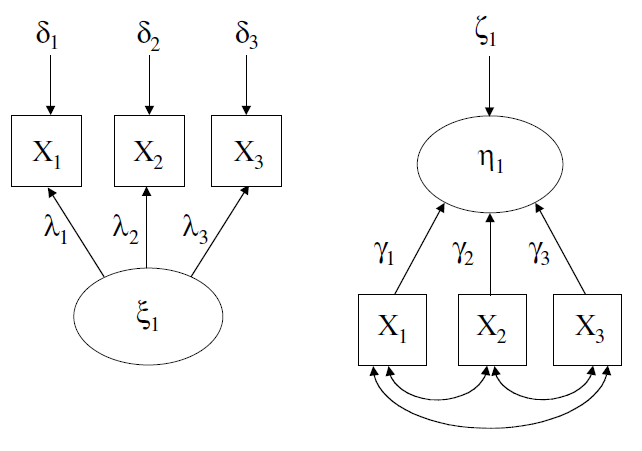
\includegraphics[scale=0.5]{chunks/borsboom}
\par\end{centering}

\caption{\label{fig:dag}(left) A reflexive model where the latent variable $\xi_{1}$ causes the observed $X_{i}$s. (right) A formative model where $\eta_{1}$ is defined in terms of the $X_{i}$s. This figure is taken from \textcite[p. 61]{Borsboom2005-iq}.}
\end{figure}

When we have a psychometric model such as the one-factor model, we want to estimate the latent $Z$. Disregarding potential covariates $X$, an estimator of $Z$ must be based on the vector of observed variables $Y$ only. That is, $\hat{Z}=\phi(Y)$, a function of the observed variables $Y$. For generalized item response models, the maximum likelihood estimator of $Z$ or its posterior mean are common estimators of $Z$. These quantities are only defined when we make parametric assumptions about all random variables involved. But the linear one-factor model is a semi-parametric model, and the maximum likelihood estimator of $Z$ need not exists. The most widely used estimator of $Z$ in psychology is the \emph{sum
score}, $\hat{Z}=\sum_{i=1}^{k}Y_{i}$, and the mean squared error-optimal linear combination $\hat{Z}=\sum_{i=1}^{k}v_{i}Y_{i}$ is popular too. Both of these make sense mainly in the linear one-factor model. 

The three fundamental questions of psychometrics are:
\begin{enumerate}
\item \textbf{Model fit}. Is the model a good approximation to reality? Are the structural and parametric assumptions defensible? Model fit in structural equation modelling is usually evaluation through model fit indices, for instance $\chi^{2}$-tests. \parencite[Chapter 15]{Mulaik2009-gc}.
\item \textbf{Reliability}. Is $\hat{Z}$ a good estimator of $Z$, assuming the model is correct? If so, the estimator is reliable. In the linear one-factor model, the reliability is most often measured by calculating coefficient alpha \parencite{Cronbach1951-in}, a statistic related to the squared correlation $\Cor^{2}(Z,\hat{Z})$. between $Z$ and $\hat{Z}$ when $\hat{Z}$ is a sum-score.
\item \textbf{Validity}. Is $Z$ what we want it to be? Even if the model is correct, $Z$ might be something else than what we would like it to be. For instance, the five questions of Table \ref{tab:IPIP} should be related to the personality trait agreeableness. But is true? Maybe they measure some other psychological trait, such as irritability, intelligence, or even a physical trait such as height. Assuming personality traits such agreeableness exists, which not every psychometrician agrees with, there are some methods to check this. The techniques are often extrastatistical, and the application of them is called \emph{validation}. \parencite[Chapter 6]{Borsboom2005-iq}
\end{enumerate}

\subsection{Reliability}

There is a mismatch between the mathematical definition of reliability and what psychologists think reliability is. The common definition of reliability is slightly different from correlation-based definition above. In our terminology, \textcite[Equation 3]{Raykov2019-yr} defines the reliability of $\hat{Z}$ as a measurement of $Z$ as
\begin{equation}
\rho=\frac{\Var Z}{\Var\hat{Z}}\label{eq:rakov-reliabiliy}
\end{equation} Under the linear model \eqref{eq:one-factor model}, $\rho = \Cor^2(Z,\hat{Z})$ when $Z$ is a linear predictor of $Z$ with zero mean, which happens when $Z$ is the sum-score $\hat{Z}=\sum_{i=1}^{k}Y_{i}$ or the mean squared error-optimal linear combination $\hat{Z}=\sum_{i=1}^{k}v_{i}Y_{i}$.

Both the correlation and ratio of variance definitions of reliability are straight-forward. Both are defined relative to statistical model, and both inform us about the quality of $\hat{Z}$ as a predictor of $Z$. But it is common for psychologists to hope for much more. For instance, \textcite{McNeish2018-vu} wrote that
\begin{quote} 
[...] researchers often report a measure of reliability to demonstrate that the items composing the measure are reliable, meaning that the scores based on the items are reasonably consistent, the responses to the scale are reproducible, and that responses are not simply comprised of random noise. Put another way, a reliability analysis provides evidence that the scale is consistently measuring the same thing [...]
\end{quote}

It is hard to reconcile all these claims with the definition of reliability, except that the responses cannot be random noise only. The claim that reliability analyses provide evidence that the scale consistently measure the same thing makes some researchers call reliability coefficients measures of internal consistency. This notion is incorrect, as the reliability coefficient cannot be used to differentiate between factors model with one or more factors \parencite[]{McDonald1981-xz}.

I do not claim that reliability coefficients are useless. If you have reason to believe in your model, a high reliability coefficient is nice to have, as it allows you to predict $Z$ well. But just as $R^2$, it is not a measure of model fit \parencite{Helland1987-eb}. Just as the $R^2$ can be small even if the linear model fits exactly, the reliability coefficient can be small even when the responses to the scale are reproducible and the scale measures the same thing. 

Reliability coefficients are ubiquitous in psychology. The most used coefficient is coefficient alpha, also known as Cronbach's alpha. This coefficient is the reliability for the sum-score under the linear one-factor model \eqref{eq:one-factor model} assuming $\tau$-equivalence, i.e., $\lambda_i = \lambda_j$ for all $i,j$. Its definition is 
\begin{equation}
\hat{\alpha}=\frac{k}{k-1}\left(1-\frac{\tr{S}}{\boldsymbol{1}^{T}S\boldsymbol{1}}\right),\label{eq:sample coefficient alpha}
\end{equation}
where $k$ is the size of $Y$, the vector $\boldsymbol{1}$ is a $k$-ary vector of only ones, and $S$ is the covariance matrix of $Y$. It is straight-forward algebra to verify that coefficient alpha equals the reliability for the sum-score $\hat{Z}$ under the $\tau$-equivalent model.

Cronbach's \citeyear{Cronbach1951-in} paper on coefficient alpha has $45673$ Google scholar cites as of August 2020. It is the third-most cited paper in psychology and in the top-hundred of the most cited papers in any field \parencite{McNeish2018-vu}. Whenever a reliability coefficient is reported, there is a $75\%$ chance it's coefficient alpha.

Reliability coefficients are routinely reported in investigations of psychometric scales. For example, \textcite{Marx1978-rf} administered \enquote{three self-report measures of self-concept} to \enquote{488 sixth grade children as the basis for a [...] self-concept measurement.} They found that the first self-report measure had sample coefficient alpha $0.56$, the second $0.55$, and the third $0.67$. 
Reliability coefficients are frequently debated by psychologists and psychometricians. A decent introduction to the literature is McNeish's \citeyear{McNeish2018-vu} attack on coefficient alpha together with the comments of \textcite{Raykov2019-yr} and \textcite{Savalei2019-se}. Psychometrika Volume 74, Issue 1 of 2009 is a relatively recent issue devoted mainly to coefficient alpha. A potential difficulty for statisticians trying to enter this fields are the two cultures of psychometrics, discussed by e.g. \textcite{Borsboom2005-iq}. One one hand are researchers working in the framework of latent variables, which is accessible to statisticians, as they work with explicit statistical models. But the majority of psychologists have been trained in the classical test theory of \textcite{Lord1968-ax}, which is slightly more esoteric to a statistician. Luckily, classical test theory can be subsumed under latent variable theory without much work.

\subsection{Normal-ogive models}
\label{subsec:Normal-ogive models}

A probit regression can written down as
\begin{eqnarray*}
Z_{i}\mid X_{i} & \sim & \beta^{T}X_{i}+\epsilon_{i}\\
Y_{i}\mid Z_{i} & \sim & 1[Z_{i}>0]
\end{eqnarray*}
provided only that $\epsilon_i$ is standard normal. Here we have a latent continuous variable $Z_i$, never observed, that captures the true regression relationship with $X$. Sadly, we only observe $Y_i$, with the associated loss of power. Probit regression is not alone in having this interpretation, as the famous logit model has the same interpretation, but with a logistically distributed $\epsilon_i$ in place of the normally distributed $\epsilon_i$. These models are popular, likely because the make more sense for binary data than the obvious competitor, linear regression.

Most psychometric data is on a Likert scale, usually on the range $1$ -- $5$ or $1$ -- $7$. These data are ordinal, and we are usually not justified in interpreting them as real numbers with the ordinary distance metric. But the popular linear factor model is best understood as modelling real numbers. How can we reconcile the linear factor model with Likert scale items?

The most common answer is to pretend the Likert scale items are real numbers, and use the linear factor model directly. Another popular answer is to use thresholding as in the probit and logit model.  

Recall the linear factor model
\begin{equation}
X=\Lambda Z+\Psi^{1/2}\epsilon,      \tag{\ref{eq:one-factor model}}
\end{equation}
where $\Lambda$ is a matrix, $\Psi$ positive definite, and $\epsilon$ uncorrelated with $Z$. Consider the scenario when we do not observe the $X_{i}$s directly, but rather $X_{i}$s discretized into $m_{i}$ categories according to
\begin{equation}
Y_{i}=j1[\tau_{i(j-1)}\leq X_{i}\leq\tau_{ij}],\quad j = 1, \ldots,m_i. \label{eq:discretization model}
\end{equation}
Here $-\infty=\tau_{i0}<\tau_{i1}<\ldots<\tau_{im_{i}}=\infty$
are thresholds for each $i$, 

If $X$ is multivariate normal, model (\ref{eq:discretization model})
is a \textit{normal-ogive model} \parencite{Swaminathan2016-rg}, also known as a discretized factor analysis model \parencite{Takane1987-pq}. Estimating of normal-ogive models is not much more involved than estimation of linear factor models. The correlation matrix of $X$ is called the \textit{polychoric correlation matrix}, it is identified and relatively straight-forward to estimate \parencite{Olsson1979-ti}. Using this estimated correlation matrix, the parameters $\Lambda$ and $\Psi^{1/2}$ can be calculating using e.g. minimum square procedures. The polychoric correlation matrix can also be used as input coefficient alpha \eqref{eq:sample coefficient alpha} instead of the sample covariance matrix, yielding the \textit{ordinal alpha} \parencite{Zumbo2007-ap}. 

Be aware that it is impossible to verify the distribution assumptions about $X$, as we do not observe it, only $Y$. While some distributions of $X$ are incompatible with normality, there are a plethora of distributions compatible with $X$ that are not normal even when $X$ is compatible with normality \parencite{Foldnes2020-ma}. In this regard, testing $X$ for normality is impossible in the same sense as non-parametric testing of the mean from Theorem \ref{thm:bahadur-savage}.
    \section{Partial identification}

Sometimes we cannot say much about how the world is. If I tell
you that $\cos x=1$ you would be at a loss to tell me exactly what
$x$ is. You could say that $x=2\pi n$, for some integer $n$, but
not anything else. The situation is bad, but could have been worse.
You do know something about $x$ after all; in the worst case scenario,
you would only know that $x\in\mathbb{R}$. You have \emph{partially
identifed} $x$. In contrast, if I tell you that $x\in[0,1]$, you
can immediately answer that $x=0$, and you have \emph{identified}
$x$.

In general, identification is about answering questions on the form
``I know $K$ but want to know $W$, to what extent is this possible?''.
If this is possible for every $K$, there is a function $K\mapsto W$,
such as $f(K)=K^{2}$. Often tough, there are multiple possible $W$
compatible with $K$, and the mapping $K\mapsto\{W\}$ is set-valued,
such as $f(K)=\{\pm\sqrt{K}\}$.

Most identification problems in statistics and adjacent fields can
be analyzed using four spaces.
\begin{enumerate}
\item $\mathcal{F}$: A space of distributions. Think of these as latent
distributions underlying some phenomenon. 
\item $\mathcal{K}$: The space of what you know. This can be a multivariate
distribution, a set of marginal distributions, or perhaps some moments
of a distribution. Will demand that $K\in\mathcal{K}$ is the image
of an $F\in\mathcal{F}$ under some function. That is, there is a
surjective function $\mathcal{F}\to\mathcal{K}$. 
\item $\Theta$: The parameter space of $\mathcal{F}$,
endowed with a surjective function $\Theta\to\mathcal{F}$. The parameter
space will sometimes contain information that cannot be deduced from
$\mathcal{F}$ itself, that is, the mapping $\theta\mapsto F$ does
not have to injective. 
\item $\mathcal{W}$: The space of what you want to know. The quantity we wish to know is a function of $\theta$, hence there is a surjective
function $\mathcal{F}\to\mathcal{K}$. 
\end{enumerate}
The mappings above induce a set-valued map $H:\mathcal{K}\to\mathcal{W}$,
the\emph{ identification region} for $F$ \parencite{Manski2003-aq}.
Figure \ref{fig:partial identifiaction situation-1} shows the situtation
using a commutative diagram. 

\begin{figure}
\noindent \begin{centering}
\[
\begin{tikzcd}
\mathcal{F} \arrow[twoheadrightarrow]{r} & \mathcal{K} \arrow[dashed]{d}{H} \\
\Theta      \arrow[twoheadrightarrow]{u} \arrow[twoheadrightarrow]{r}  & \mathcal{W}
\end{tikzcd}
\]
\par\end{centering}
\caption{\label{fig:partial identifiaction situation-1}The situation of partial
identification analysis. The double-headed arrows ($\twoheadrightarrow$)
denote surjections, the dashed arrow ($\protect\dashrightarrow$)
denotes the induced map.}
\end{figure}

Identification analysis is usually not presented in this formal way,
but is fruitful for three reason. First, it makes a clear that there is a connection
between the seemingly disparate uses of the word ``identification''
across the stastical, medical, econonomic and sociological literutures.
Second, it allows us to state results using little notation and words.
For instance, $H(K)\subseteq A$ means that $A$ contains the identification
region of $K$, when $K$ is what we know. Third, it is possible to prove some general results
about these problems.

As is customary in partial identification analysis, we ignore sampling
error \parencite{Manski2003-aq}. Making this assumption reduces the complexity
of the problem a lot. 

Identification analyses come in three forms, depending on which of maps the maps in Figure \ref{fig:partial identifiaction situation-1} are identities. 
\begin{description}
\item [{Convenience~identification}] When statisticians talk about identifiability they usually think about convenience. Unidentified parameters make estimation difficult and is a prerequisite for most asymptotic results. In this case, the interpretation of the parameters are often of no consequence. Both $\Theta\to\mathcal{W}$ and $\mathcal{F}\to\mathcal{K}$ are identity maps. We know $F$ and wish to know $\theta$. 
\item [{Partial~identification~of~distributions}] When $\Theta$ can be identified with the space of distributions $\mathcal{F}$, we are dealing with partial identification of distributions. In this setting, $F\in\mathcal{F}$ is the true, latent distribution, but we only observe some $K=\Psi(F)$. We are usually not interested in getting to know $F$ itself, but rather some summary such as a correlation. A famous example is the error-in-variables regression problem, considered below.
\item [{Structural~parameters}] Sometimes you want to say something about parameters that are in extra-probabilistical, that is, they cannot be encoded by probability measures. In problems of this type the spaces $\Theta$ and $\mathcal{F}$ are distinct. The most famous example is causal inference, where different causal assumptions can produce identical joint distributions. 
\end{description}

\subsection{Convenience identification}

Identification is usually about parameterizations. A parameterization is just a convenient way to represent an object, and we usually want each representation to be unique. We want parameterizations since probabilities is difficult beast to work with directly, but tuples of reals are easy to handle. Let $\mathcal{P}$ be family of probability measures and $\theta:\text{\ensuremath{\Theta\to\mathcal{P}}}$ a surjective function on some parameter space $\Theta$. We will call $\theta$ a parameter and say it is\emph{ identified }if $\theta$ is injective. 
\begin{example}
\label{exa:normal unidentified}Let $\Theta=[0,\infty)$ and map $\theta$ to the the probability distribution of a mean-zero normal variable with standard deviation $\theta$. Then $\theta$ is injective, hence identified. On the other hand, if $\Theta=\mathbb{R}$ and $\theta$ maps to the mean-zero normal probability with standard deviation $|\theta|$, $\theta$ is not identified. For instance, both $-1,1$ maps to the the standard normal probability.
\end{example}

Parameterizing probability measures is in many cases quite important, both for interpretations and mathematics. The prior in Bayesian statistics can be formally formulated as a probability measure over probability measures. For instance, a $\textrm{Beta}(\alpha,\beta)$ prior over the $p$-parameter of a binomial binomial distribution can also be formulated as a probability measure over binomial distributions directly. We want to use nice the parameterization since we understand and are able to work with the topology of $[0,\infty)^2$ easily. Moreover, we can verify that it's topology is separably metrizable (i.e., Polish), which implies that the $\sigma$-algebra generated by its open sets is a standard Borel space \parencite{Kechris2012-nh}. Most measure theory works smoothly only for standard Borel spaces \parencite[][Chapter 1]{Van_der_Vaart1996-dx}, hence our parameterization gives us assurance we won't have unpleasant surprises such as non-measurability down the line. 

Identifiability is often a crucial technical assumption, required for the math to work. For instance, an identifiable parameterization is required for Doob's consistency theorem \parencite{Miller2018-xq} and consistency of Manski's maximum score estimator \parencite{Manski1975-gl}. Moreover, it is needed for numerical algorithms such as Newton--Raphson in order to assure convexity of the objective function.

\subsection{Partial identification of distributions}
In partial identification of probability distributions, the spaces $\mathcal{F}$ and $\Theta$ of \ref{fig:partial identifiaction situation-1} are equal. While partial identification is important in several fields, econometricians have been more active than others in studying it. Two important books are those of \textcite{Manski1999-ab,Manski2003-aq}, and \textcite{Tamer2010-rj} is a more recent review. The motivation for partial identification analyses is a principle connecting assumptions with believeability \textcite[p. 1]{Manski2003-aq}:
\begin{quote}
\emph{The Law of Decreasing Credibility: }The credibility of inference
decreases with the strength of the assumptions maintained.
\end{quote}
There is a trade-off between credibility and assumptions. Strong assumptions bring plenty of benefits, such as models that are much easier to deal with computationally and mathematically. It is easier to compute a linear regression with normal errors than one with \emph{t}-distributed errors, and confidence intervals are exact only in the former case. Moreover, adding assumptions can make models much easier to interpret; the linear regression model $Y=\alpha+\beta X+\epsilon$ is as clear as day, $Y=\alpha+\beta X+\delta e^{\sin X}\Gamma(X)\epsilon$ is obscure. 

Frequently assumptions are made only to make sure the model is identifiable, as in the following is the quintessential partial identifiability problem.
\begin{example}[Error-in-variables regression model, \textcite{Tamer2010-rj}]
Let $Y,Z$ be two variables of finite variance, $Y$ observable and $Z$ latent. We want to know $\beta=\Cov(Y,Z)/\Var(Z)$, that is, the regression coefficient of $Y$ on $Z$. Let $X=Z+\eta$ be an observed variable, where $\eta$ has finite second moments and is uncorrelated with $X$ and $Z$. We know the second moments moments $\Var X$ and $\Cov(Y,X)$, i.e., $K=(\Var X,\Cov(Y,X)$. What can we say about $\beta$? 

Define $\beta^{\star}=\Cov(X,Y)/\Var X$, the regression coefficient of $Y$ on $X$. Since $\Var X=\Var Z+\Var\eta$
and $\Cov(X,Y)=\Cov(Z+\eta,Y)=\Cov(Z,Y),$we find
\[
\beta^{\star}=\frac{\Cov(Z,Y)}{\Var Z+\Var\eta}=\frac{\beta}{1+\frac{\Var\eta}{\Var Z}}=\frac{\Var Z}{\Var X}\beta.
\]
If we make the assumption that $m\leq\Var Z\leq\Var X$, we obtain
the identification region $H=\beta^{\star}[1,\Var X/m)$. 
\end{example}

Now we will consider, in more detail, two problem of partial identification of distributions.

\subsubsection{When you know some correlations}
Let $X,Y,Z$ be random variable with unit variance. Assume you know
$\rho_{12}=\Cov(X,Y)$, $\rho_{23}=\Cov(Y,Z)$. What can you say about
$\rho_{13}=\Cov(X,Z)$? This problem is known from the literature
on matching \parencite{Rassler2012-rp}.You need to fill out
\[
\Phi=\left[\begin{array}{ccc}
1 & \rho_{12} & ?\\
\rho_{12} & 1 & \rho_{23}\\
\text{\ensuremath{?}} & \rho_{23} & 1
\end{array}\right]
\]
subject only to the constraint that $\Phi$ is positive definite. 
\begin{proposition}
\label{prop:correlation identification}The following identification
sets are true.
\begin{itemize}
\item[(i)] When $\rho_{23}$ and $\rho_{12}$ are known, the identification region
for $\rho_{13}$ is the open interval
\begin{equation}
\rho_{13}\in\rho_{12}\rho_{23}\pm\sqrt{\rho_{12}^{2}\rho_{23}^{2}-\rho_{23}^{2}-\rho_{12}^{2}+1}.\label{eq:identification set correlation}
\end{equation}
In particular, when $\rho_{12}=\rho_{23}=\rho$, the partial identification
set is $(2\rho^{2}-1,1)$. 
\item[(ii)] If only $\rho_{12}$ is known, the identification region for $(\rho_{13},\rho_{23})$
is the ellipse with width $2\sqrt{1+\rho_{12}}$ and height $2\sqrt{1-\rho_{12}}$,
rotated $\pi/4$ degrees. In particular, when $\rho_{12}=0$, the
identification set is the open Euclidean unit ball in $\mathbb{R}^{2}$.
\end{itemize}
\end{proposition}

\begin{proof}
We will use Sylvester's criterion \parencite{Gilbert1991-ch}. Applied
to a $3\times3$-matrix $A$, it says that $A$ is positive definite
if and only if (i) $A_{11}$ is positive, (ii) the determinant of
the $2\times2$ upper-left corner of $A$ is positive, and (iii) the
determinant of $A$ itself is positive. 

Since $\Phi_{11}=1$, (i) satisfied, and so is (ii) since $\rho_{12}$
is a correlation. The determinant of $\Phi$ is
\begin{eqnarray*}
\det\Phi & = & (1-\rho_{23}^{2})-\rho_{12}(\rho_{12}-\rho_{23}\rho_{13})+\rho_{13}(\rho_{12}\rho_{23}-\rho_{13}).
\end{eqnarray*}
Fixing $\rho_{12}$ and $\rho_{23}$, this is positive and if the
quadratic functin $\rho_{13}^{2}-2(\rho_{12}\rho_{23})\rho_{13}+(\rho_{23}^{2}+\rho_{12}^{2})<0$.
Since this equation has roots $\rho_{12}\rho_{23}\pm\sqrt{\rho_{12}^{2}\rho_{23}^{2}-\rho_{23}^{2}-\rho_{12}^{2}+1}$,
equation (\ref{eq:identification set correlation}) follows. As for
$\rho_{12}=\rho_{23}=\rho$, the limits are $\rho^{2}\pm\sqrt{(\rho^{2}-1)^{2}}$,
or, equivalently, $(2\rho^{2}-1,1).$

Time to take on (ii). Fix $\rho_{12}=\rho$ and define $x=\rho_{13},y=\rho_{23}$.
Then equation (\ref{eq:identification set correlation}) can be rearranged
to
\begin{equation}
y=x\rho+\sqrt{1-\rho^{2}}\sqrt{1-x^{2}}.\label{eq:ellipse eq1}
\end{equation}
Subtracting $x\rho$ on both sides and squaring yields $(y-x\rho)^{2}=(1-\rho^{2})(1-x^{2}).$
In expanded form, this is $y^{2}-2xy\rho+x^{2}\rho^{2}=1-\rho^{2}-x^{2}+x^{2}\rho^{2}$,
which can be rearranged to $y^{2}-2xy\rho+x^{2}=1-\rho^{2}$. 

The formula for an ellipse with width $2a$ and height $2b$, rotated
$\theta$ degrees is

\[
\frac{(x\cos\theta+y\sin\theta)^{2}}{a^{2}}+\frac{(x\sin\theta-y\cos\theta)^{2}}{b^{2}}=1.
\]
When $\theta=\pi/4$, $\cos\theta=\sin\theta=1/\sqrt{2}$, hence 
\begin{equation}
\frac{(x+y)^{2}}{2a^{2}}+\frac{(x-y)^{2}}{2b^{2}}=1\label{eq:pi/4-rotated ellipse}
\end{equation}
is the ellipse with width $2a$ and height $2b$ rotated $\theta=\pi/4$
degrees.

Take $a=\sqrt{1+\rho_{12}}$ and $b=\sqrt{1-\rho_{12}}$ and plug
them into (\ref{eq:pi/4-rotated ellipse}) to verify it is equivalent
to $y^{2}-2xy\rho+x^{2}=1-\rho^{2}$. Since each $x,y$ in the ellipse
will satisfy the limits of (\ref{eq:identification set correlation}),
we are done.
\end{proof}
\begin{figure}
\noindent \begin{centering}
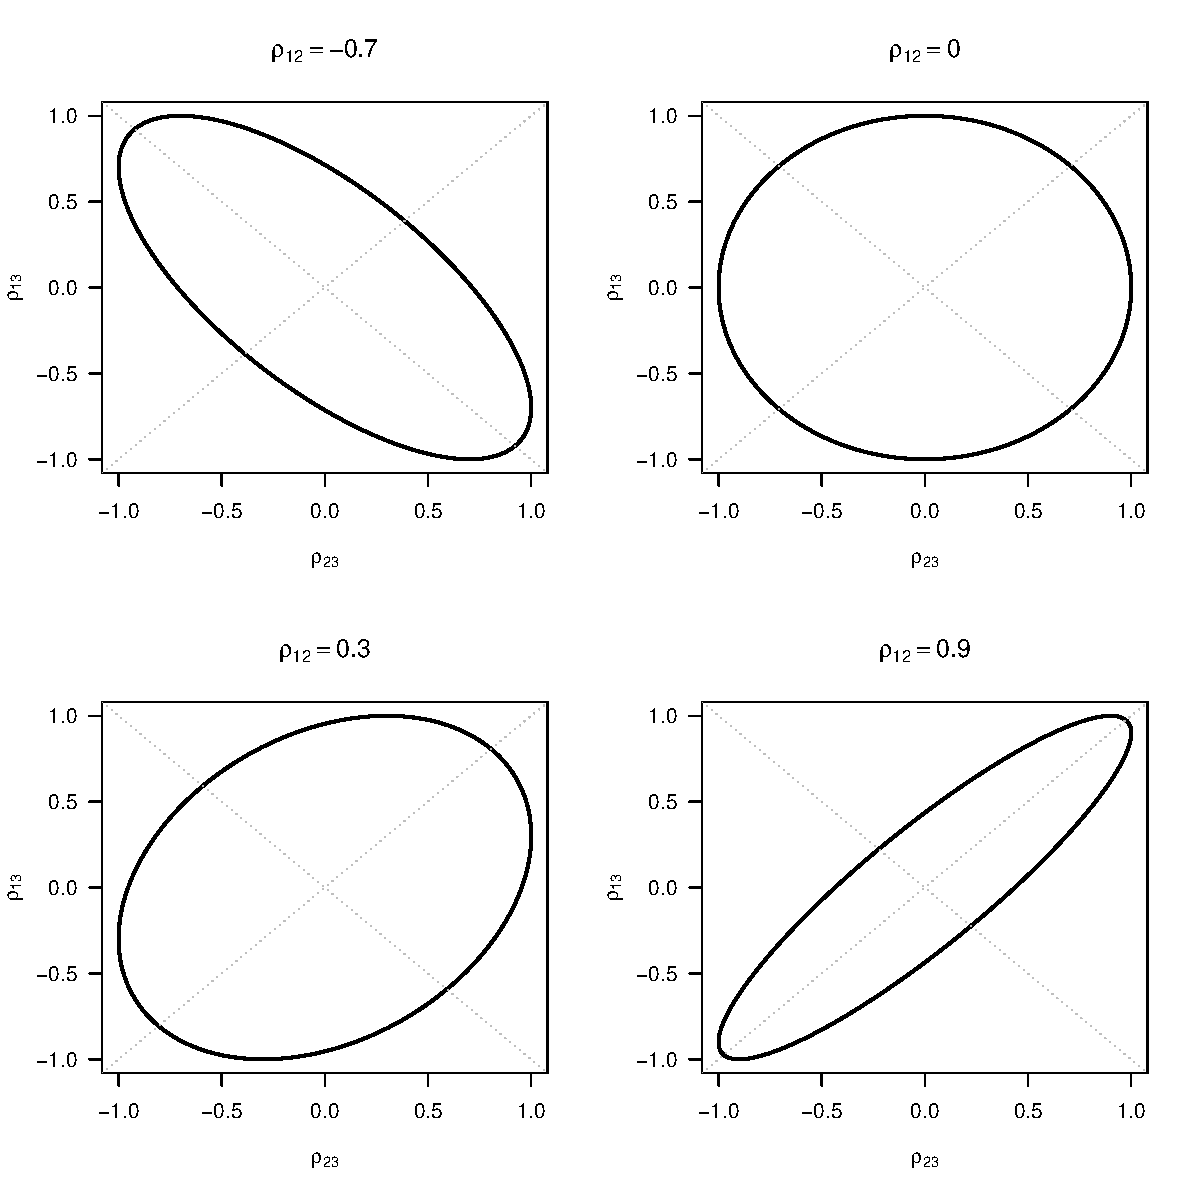
\includegraphics[scale=0.4]{chunks/rho}
\par\end{centering}
\caption{The ellipses of Proposition \ref{prop:correlation identification}
for a selection of correlations $\rho_{12}$.}
\end{figure}
%
\begin{example}[{\textcite[p. 10]{Rassler2012-rp}}]
 Assume 
\[
\Phi=\left[\begin{array}{ccc}
1 & 0.9 & \rho_{13}\\
0.9 & 1 & 0.8\\
\rho_{13} & 0.8 & 1
\end{array}\right]
\]
Applying Propositon \ref{prop:correlation identification} gives us
the identification set $(0.4585,0.9815)$ for $\rho_{13}$.
\end{example}


\subsubsection{How many people know basic scientific facts?}
\begin{quote}
\textbf{\emph{Question 3}}: Does the Earth go around the Sun, or does
the Sun go around the Earth?

\medskip

$\bigcirc$ Earth goes around the Sun.

$\bigcirc$ Sun goes around the Earth.
\end{quote}
The National Science Board \citeyear[Table 7-8]{National_Science_Board2014-yl}
reports that a shockingly high percentage of people answer this question incorrectly. Only $74$\% of American adults answered correctly, while an even worse $66$\% of adults in the European Union answered correctly. South Koreans did slightly better, at $86$\%. But the true percentage of Americans who know the Earth goes around the Sun is probably even lower than $74$\%. For a non-human monkey would select either option with equal probability, and some humans probably do this too. The base-line of no knowledge is $50$\% correct answers, and we haven't corrected for this. So what's the real percentage of people of who knows that the Earth goes around the Sun? 

A popular way to model people's state of knowledge is to use probability distributions. Imagine everyone has a probability distribution over the answers to Question 3. Denote this distribution $c$ and the proposition that the Earth goes around the Sun by $A$. Then the knowledge of a person is captured by $c(A)$. In philosophy, this is called a \emph{credence function} \parencite{Pettigrew2019-rk}.

We want to know the percentage of people that knows the answer to $A$. Even if we knew everyone's credence function $c$, the answer to this question is not completely straightforward. Knowing or not knowing must involve a cutoff. For instance, you could claim that you know $A$ when you are at least $95\%$ certain of $A$ and $A$ is true. This cutoff is arbitrary, and could equally well have been $75\%$, $99\%$, or anything else. A natural restriction is to demand a certainty of more than $50\%$, but otherwise any percentage appears defensible. To take this arbitrariness of the cutoffs into account, let us say that a person $\alpha$-knows $A$ if $c(A)>\alpha$ and $A$ is true. Now we can restate goal: We want to find the percentage of the population that $\alpha$-knows that the Earth orbits the sun.

To model all of this, let $c$ be a credence function sampled according to $Q$ and $X\mid c$ sampled according to $c$,
\[
c\sim Q,\quad X\mid c\sim c.
\]
The next step is to decide on the possible space of distributions $Q$. \textcite[Chapter 2, endnote 28]{Caplan2018-oj} assumes that every person either knows $A$ with certainty or guesses with $50/50$ odds.
In this case, $Q$ can be a parameterized by $\gamma$, the proportion who knows for certain. Then $1-\gamma=2(1-P(A))$, hence $\gamma=1-2(1-P(A))=2P(A)-1$. When $P(A)=0.74$ we get $\gamma=0.48$, hence just below $50\%$ of the population $\alpha$-knows the Earth goes around the Sun when $\alpha\geq0.5$. But this assumption doesn't look quite right, for why would there be no one who are, say, $90\%$ certain that the Sun goes around the Earth?

In the spirit of \textcite{Manski2003-aq}, we will make no assumption about $Q$. Let $H_\alpha(\beta)$ be the identification region for $\alpha$-knowledge of Question 3 when $P(X=1) = \beta$. Then we get the following proposition.
\begin{proposition}
\label{prop:guessing regions}Let $P(X=1)=\beta\in(0,1)$. Then 
\[
H_{\alpha}(\beta)=\begin{cases}
[(\beta-\alpha)/(1-\alpha),1], & \textrm{when }\beta>\alpha,\\
(0,1), & \textrm{when }\beta=\alpha,\\{}
[0,\beta/\alpha], & \textrm{when }\beta<\alpha.
\end{cases}
\]
\end{proposition}

\begin{proof}
Assume $\beta>\alpha$. Let $A$ be the event that $c(1)\leq\alpha$
and $B$ the event that $c(1)>\alpha$. Denote $P(X=1\mid A)=\alpha-\epsilon$,
where $\epsilon\in[0,\alpha]$, assume $P(X=1\mid B)=\beta+\delta$,
$\delta\in[0,1-\beta]$, and denote $P(B)=q$. By the law of total
probability,
\[
P(X=1)=P(B)(\beta+\delta)+P(A)(\alpha-\epsilon).
\]
Since $\beta=P(X=1)$, $P(B)=q$, and $P(A)=1-q$, we get $\beta=q(\beta+\delta)+(1-q)(\alpha-\epsilon).$
Rearrange to get $q=(\beta-\alpha+\epsilon)/(\beta-\alpha+\epsilon+\delta)$.
This is maximized when $\delta=0$, when $q=1$. It is minimized when
$\epsilon=0$ and $\delta=1-\beta$, when $q=(\beta-\alpha)/(1-\alpha).$

That $E(\alpha)=(0,\beta/\alpha]$ when $\alpha\geq\beta$ can be verified by duality. For now $1-\alpha\leq 1-\beta$, and we can use the same analysis as above when regarding $2$ as the right answer. Hence the maximum is $1$ and the minimum is $(1-\beta-(1-\alpha))/(1-(1-\alpha)=(\alpha-\beta)/\alpha$. Turn back to the case when $1$ is the right by forming $1-(0,(\alpha-\beta)/\alpha)=(0,\beta/\alpha].$
\end{proof}
\begin{figure}
\noindent \begin{centering}
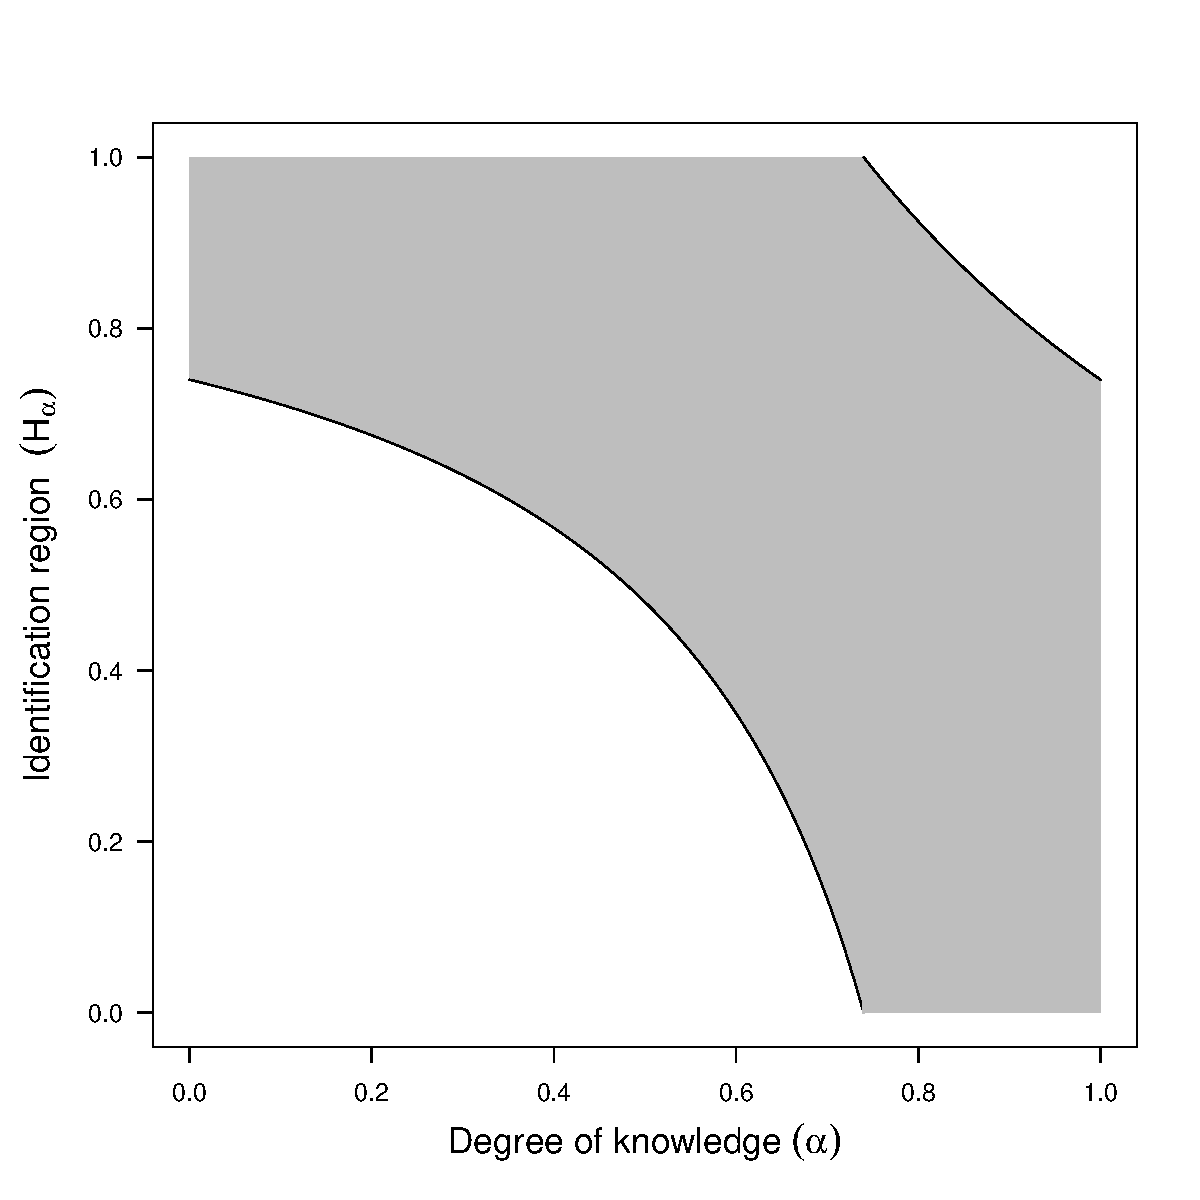
\includegraphics[scale=0.5]{chunks/knowing}
\par\end{centering}
\caption{\label{fig:Identification-regions-guessing}Identification regions
when $P(A)=0.74$.}
\end{figure}

The identification regions of Proposition \ref{prop:guessing regions} are wide. Figure \ref{fig:Identification-regions-guessing} tells the story when $P(A)=0.74$. In particular, when $\alpha=0.95$, we get $E(\alpha)=[0,0.78]$, meaning anything between $0\%$ and $78\%$ of the population knows $A$ with minimum $95\%$ certainty. If we choose the low $\alpha=0.6$, we get $E(\alpha)=[0.35,1]$, so at least $35\%$ of the population knows $A$ with minimum $60\%$ percent certainty. In conclusion, we can't really say how many Americans know the Earth orbits the Sun.

\subsection{Identification of structural parameters}

Structural parameters are extra-probabilistical; they encode something
about the world the isn't captured in any probability distribution.
Causal inference is about structural parameters; the joint distribution
of $(X,Y)$ does not tell us if $X$ causes $Y$. The causal information
is encoded in e.g. a causal graph \parencite{Pearl2009-zf} or a system
of counterfactuals \parencite[Chapter 4]{Pearl2016-tc}. A related example
of identifacation of structural parameters is from psychometrics.
In general, several structural equation models can give rise to exactly
the same joint distribution, but with highly disparate interpretations
\parencite{Raykov2001-ap}. Econometrics have perhaps the most famous
identification problem, sometimes called \textit{the identification problem in econometrics} \parencite{Manski1999-ab}.
\begin{example}[The identification problem in econometrics]
 Let $p$ be the price and $q$ the quantity of some good. Assume
the linear supply and demand functions
\begin{eqnarray*}
s(p) & = & \alpha_{s}+\beta_{s}p+\epsilon_{s}\quad\textrm{(supply)},\\
d(p) & = & \alpha_{d}+\beta_{d}p+\epsilon_{d}\quad\textrm{(demand).}
\end{eqnarray*}
Here $s(p)$ is the quantity supplied at the price $p$, $d(p)$ is
the quantity demanded at the price $p$, and $\epsilon_{1},\epsilon_{2}$
are uncorrelated error terms with zero mean and variances $\sigma_{1}^{2},\sigma_{2}^{2}$.
If prices are in equilibrium, $q=s(p)=d(p)$, hence
\[
q=\alpha_{s}+\beta_{s}p+\epsilon_{1}=\alpha_{d}+\beta_{d}p+\epsilon_{2}.
\]
We want to know the supply and demand functions, or equivalently,
$(\alpha_{s},\beta_{s},\alpha_{d},\beta_{d})$. We know the mean $\mu$
and covariance $\Sigma$ of $(p,q)$:
\begin{eqnarray*}
\mu & = & \left(\frac{\alpha_{d}-\alpha_{s}}{\beta_{s}-\beta_{d}},\frac{\beta_{s}\alpha_{d}-\beta_{d}\alpha_{s}}{\beta_{s}-\beta_{d}}\right)\\
\Sigma & = & \frac{1}{(\beta_{s}-\beta_{d})^{2}}\left[\begin{array}{cc}
\sigma_{1}^{2}+\sigma_{2}^{2} & \beta_{d}\sigma_{1}^{2}+\beta_{s}\sigma_{2}^{2}\\
\beta_{s}\sigma_{1}^{2}+\beta_{s}\sigma_{2}^{2} & \beta_{d}^{2}\sigma_{1}^{2}+\beta_{s}^{2}\sigma_{2}^{2}
\end{array}\right]
\end{eqnarray*}
Here we have $5$ knowns $(\mu_{1},\mu_{2},\Sigma_{11},\Sigma_{22},\Sigma_{12})$
and $6$ unknowns $(\alpha_{s},\beta_{s},\alpha_{d},\beta_{d},\sigma_{1}^{2},\sigma_{2}^{2})$
in a system of quadratic equations. This system of equations has no
unique solution. To rectify this, several identifying restrictions have been proposed. See \textcite[Chapter 6]{Manski1999-ab} for details.
\end{example}
    \printbibliography[heading = subbibliography]

    \paper              % "Chapter" is renamed "Paper"
    \paperpage          % Similar to \part*{Papers}, but appears in TOC
    \numberofpapers{3}  % Specify size of thumb indices

    %\documentclass{standalone}

% Standalone ensures that
% everything from \documentclass to \begin{document}
% in this document is ignored when included by main.tex.

\begin{document}

\author
{
    First Author
    \and
    Second Author
}
\title{The Second Chapter}
\thanks{The authors were partially supported by CERN.}
\metadata
{
    Published in \emph{Journal of Universal Rejection},
    June~2011,
    volume~3,
    issue~2,
    pp.~123--456.
    \doi{10.1000/182}.
}
\maketitle
\label{pap:second}

\begin{abstract}
    \kant[7]     % Dummy text
\end{abstract}

\startcontents[chapters]
\printcontents[chapters]{}{1}{\section*{\contentsname}}

\section{Introduction}

\kant[8-11]      % Dummy text

\begin{theorem}[{\cite[95]{AM69}}]
    \label{thm:dedekind}
    Let \( A \) be a Noetherian domain of dimension one. Then the following are equivalent:
    \begin{enumerate}
        \item
        \( A \) is integrally closed;

        \item
        Every primary ideal in \( A \) is a prime power;

        \item
        Every local ring \( A_\mathfrak{p} \) \( (\mathfrak{p} \neq 0) \) is a discrete valuation ring.
    \end{enumerate}
\end{theorem}

\begin{acknowledgements}
    The first author was partially supported by The Research Council of Norway.
\end{acknowledgements}

%% Format bibliography like a section, not a chapter:
\printbibliography[heading = subbibliography]
\stopcontents[chapters]

\paragraph{Authors' addresses}
\begin{description}
    \item[First Author]
    University of Oslo,
    Postboks 1337 Blindern, 0316 Oslo, Norway,
    \href{mailto:fauthor@uio.no}{fauthor@uio.no}

    \item[Second Author]
    Oxbridge University,
    221B Baker Street, London NW1 6XE, United Kingdom,
    \href{mailto:second.author@oxbridge.co.uk}{second.author@oxbridge.co.uk}
\end{description}

\end{document}
    %\documentclass{standalone}

% Standalone ensures that
% everything from \documentclass to \begin{document}
% in this document is ignored when included by main.tex.

\begin{document}

\author
{
    First Author
    \and
    Second Author
}
\title{A4 paper}
\metadata{Submitted for publication. \arxiv{1708.04101}.}
\maketitle
\label{pap:A4}


\includearticle{sections/a4paper}

\end{document}
    %\documentclass{standalone}

% Standalone ensures that
% everything from \documentclass to \begin{document}
% in this document is ignored when included by main.tex.

\begin{document}

\author{First Author\protect\footnotemark}
\title{The Fourth Chapter}
\metadata{To appear in \emph{Journal of Universal Rejection}.}
\maketitle
\label{pap:fourth}

\footnotetext
{%
    University of Oslo,
    Postboks 1337 Blindern, 0316 Oslo, Norway,
    \href{mailto:fauthor@uio.no}{fauthor@uio.no}
}

\begin{abstract}
    \kant[12] % Dummy text
\end{abstract}

\section{First Section}
\kant[13-14]  % Dummy text

\begin{subappendices}             % Appendix for this chapter/paper only
    \section{First Subappendix}
    \label[appendix]{sec:sub-app} % Optional argument: Correct cross reference
    \kant[15]                     % Dummy text
\end{subappendices}

\begin{acknowledgements}
    Thanks to the anonymous referee for pointing out that \cref{sec:sub-app} can be found in \cite{Har77}.
\end{acknowledgements}

%% Format bibliography like a section, not a chapter:
\printbibliography[heading = subbibliography]

\end{document}

    %\appendix           % "Chapter" is renamed "Appendix"
    %\appendixpage       % Similar to \part*{Appendices}, but appears in TOC

    %\chapter{The First Appendix}
\label{app:first-app}
\kant[20-21] % Dummy text
\section{First Section}
\kant[22]    % Dummy text
\section{Second Section}
\kant[23-24] % Dummy text
    %\chapter{Source Code}
\label{app:source}
\section{Implementation}
The \texttt{phduio} class is implemented in the following way:
\lstinputlisting[language = {[LaTeX]{TeX}}]{phduio.cls}

\end{document}